%======================================================================
\chapter{Zupply Framework Design} \label{ch:zupply-design}
%======================================================================

\section*{Declaration of Contributions}
This chapter is based on \cite{Badakhshan2024Zupply}. I am the sole author of this chapter under the supervision of Professor Guang Gong.



\section{Introduction}


The Zupply framework facilitates the authenticated and privacy-preserving, decentralized maintenance of directed acyclic graphs (\gls{dag}s). \gls{dag}s, which are pivotal in representing data flows, find utility in diverse applications. One notable application is in supply chain management (\gls{scm}), where a \gls{dag} is instrumental in tracking a product's progression. In this context, each \gls{dag} node represents a unique stage in the product's lifecycle, facilitating an understanding of the sequence and interdependencies of these stages. \gls{dag} data structure has the flexibility to either extend a sequence, divide it into two, or merge two sequences into one. Beyond \gls{scm}, \gls{dag} structured data (or simply \gls{dag}) is also employed in various other domains, including version control systems (\gls{vcs}) (e.g., Git \cite{gitonline2023} and Mercurial \cite{mercurial}). Proposing a practical, fully decentralized, and trustless scheme for maintaining \gls{dag} that simultaneously preserves the privacy of entities creating data records and ensures the authentication of these records addresses significant challenges in current \gls{scm} solutions.

\gls{scm} brings together numerous entities, from suppliers to consumers, requiring the secure flow of items, information, and funds \cite{wisner2021principles}. Ensuring product quality and origin compliance necessitates transparent traceability \cite{SUN2019658}, but protecting private information and trade secrets is equally vital, especially for smaller enterprises \cite{ Winter2023SMEs}. Existing systems often rely on centralized authorities or permissioned blockchains, which are neither fully trustless nor decentralized. Permissionless (public) blockchains create a trustless environment, but their full transparency and high on-chain storage costs pose challenges \cite{ Zhou2022EthereumGraph}. Although solutions based on 
interplanetary file system (\gls{ipfs}) \cite{Benet2014} can address storage issues, they lack privacy-preserving authentication \cite{Khor2023, Musamih2021}. 

We are proposing a universal \gls{scm} framework that meets various requirements, such as transparency, agility in collaboration, and affordability for micro, small and medium enterprises (\gls{msme}s). To achieve this, we suggest designing an \gls{scm} system that uses public blockchains. This system aims to provide cost-efficient solutions by using off-chain storage for product histories while ensuring data integrity and authenticity. This way, all supply chain participants, including end consumers, can verify a product's history. Since products often comprise materials from various sources, we recommend using \gls{dag} structured data to manage multi-sourced products, enhancing traceability and efficiency. 

The trustless nature of public blockchains underpins our framework, where the authorization of entities is managed via smart contracts. This setup facilitates a fully decentralized structure, allowing for the autonomous execution of business agreements. Consequently, entities, regardless of their prior reputations, can establish trust within this immutable blockchain environment. Moreover, this system streamlines the inception of new collaborations, enabling partners to engage effortlessly and swiftly through mutual smart contract adherence. Nevertheless, the inherent transparency of public blockchains presents a challenge to privacy. 
To address these challenges, Zupply introduces anonymous authentication token (\gls{aat}), \gls{aat} ownership transfer (\gls{aatot}), and leverages off-chain storage for anonymous, affordable, transparent, and decentralized product histories while guaranteeing data authenticity and  preserving the unlinkability of collaborators. Zupply incorporates \gls{aat} and \gls{aatot} to ensure anonymity and unlinkability among entities. By employing DAG structures, it efficiently manages multi-sourced products and eliminates the need for centralized intermediaries. Zupply is the first framework enabling fully decentralized anonymous authentication for off-chain DAG data, Zupply has extensive potential beyond \gls{scm}, including \gls{vcs} and general-purpose anonymous authentication. 

\subsubsection{Our Contributions:}
\begin{enumerate}
    \item  \textbf{Zupply Framework with Enhanced Security Properties}: We utilize zero-knowledge proof (\gls{zkp}) to design a novel \gls{aat} scheme on smart contract-enabled public blockchains. Zupply includes a set of algorithms and protocols that execute on-chain unlinkable \gls{aatot} and off-chain anonymous data authentication, satisfying four main properties: (1) Anonymity: The anonymity of data uploaders and \gls{aat} owners is preserved, except for \gls{aat}s initiating a \gls{dag}. (2) Unlinkability: The link between entities collaborating in maintaining a \gls{dag}, which represents supply chain data records, is hidden. (3) Integrity: Each data record is authenticated and unaltered, allowing the auditor to verify that the data record is created solely by the authorized entity for uploading at that stage. (4) Trustlessness: Zupply operates without trusted parties during protocol execution and achieves high decentralization by relying on public blockchains.
    
    
    \item  \textbf{Off-chain Authenticated Storage}: Zupply separates storage from blockchain while maintaining a concealed link to the \gls{aat}s. This allows entities to anonymously upload data. The off-chain anonymous authentication capability decreases blockchain storage costs, enhances anonymity, and allows entities to chose their storage approach based on their specific needs for decentralization and cost. Our framework decreases blockchain storage costs mores by minimizing proof sizes and introducing a novel algorithm for Merkle hash trees  \cite{Merkle1980}.
      

\end{enumerate}


\section{Zupply Framework}
\label{sec:Zupply Framework}

\begin{table}[h]
    \centering
        \caption{The main symbols used in the Zupply framework}
    \begin{tabular}{c c}
    \hline 
        \textbf{Symbol} & \textbf{Description} \\
    \hline 
        $\tau$ & Time \\
        $e_i, \mathbf{E}_\tau$ & The $i$-th entity, the set of all $e$s at  $\tau$  \\
        $T_i, \mathbf{T}_\tau$ & The $i$-th \gls{aat}, the set of all $T$s at  $\tau$  \\
        $\texttt{cm}_i, \mathbf{C}_\tau$ & Commitment to the $i$-th \gls{aat}, the set of all $\texttt{cm}$s at $\tau$\\
        $\texttt{eol}_i, \mathbf{X}_\tau$ & End-of-life of the $i$-th \gls{aat}, the set of all $\texttt{eol}$s at $\tau$\\
        $\texttt{tx}_i, \mathbf{TX}_\tau$ & The $i$-th transaction, the set of all $\texttt{tx}$s at $\tau$\\
        $\mathsf{MHT}$, $\texttt{rt}_\tau$ & Merkle Hash Tree, the $\mathsf{MHT}$'s root at  $\tau$\\
        $d_n, \mathbf{D}_\tau$ & The $n$-th data record, the set of all $d$s at $\tau$ \\
        $\textsc{cid}_n, \mathbf{CID}_\tau$ & CID of the $n$-th data record, the set of all  $\textsc{cid}$s at $\tau$\\
        $\texttt{Tag}_i$ & Data ownership transfer tag associated with $T_i$\\
        $\mathbf{L}_\tau$ & The shared ledger at $\tau$ \\
    \hline 
    \end{tabular}
    \label{tab:Zupply-Symbols}
\end{table}

Zupply is a portmanteau of `Z' from \gls{zkp}s \cite{Goldwasser1985} and `Supply' from \gls{scm}. 
Zupply presents a novel \gls{aat} scheme, using \gls{zkp} algorithms that are efficiently managed on smart contract-compatible public blockchains (e.g., Ethereum \cite{ethereum}), including an anonymous, unlinkable \gls{aatot}. This enables the creation of authenticated records of \gls{dag}, thereby maintaining a verifiable history of products in the supply chain. At the same time, the anonymity of each entity and the unlinkability among them are preserved. Namely, any auditor can verify that a data record is authenticated (Definition \ref{def:Authenticated Data}) while the data creator remains anonymous. Additionally, no adversary may learn the collaboration between different entities and the supply chain each entity is involved with. 

The main symbols used in this chapter are listed in Table \ref{tab:Zupply-Symbols}. 
The Zupply framework comprises three primary components, as illustrated in Figure \ref{fig:Zupply-Architecture}. The following descriptions provide an overview of each component:

\begin{enumerate}
    \item \textit{Entities}: Data uploaders or auditors in the supply chain, ranging from producers to consumers, form the entity set in the Zupply Framework. Entities need to run Zupply Node (\textsc{Z-Node}).  %Each participant, after installing the Zupply Node (\textsc{Z-Node}), is responsible for uploading or auditing product data, such as temperature and location.

    \item \textit{Blockchain Platform (BP)}: Zupply operates on a smart contract-enabled, permissionless blockchain, essential for managing the Zupply smart contract ($\mathcal{C}_Z$) that enables the creation and transfer of \gls{aat}s. 

    \item \textit{Decentralized Cloud Storage (\gls{dcs})}: The \gls{dcs} utilized by Zupply is a secure, manager-less system based on IPFS \cite{Benet2014}, storing data records ($d$) addressed by content identifiers (\textsc{cid}). 
    
\end{enumerate}

\begin{figure}
    \centering
    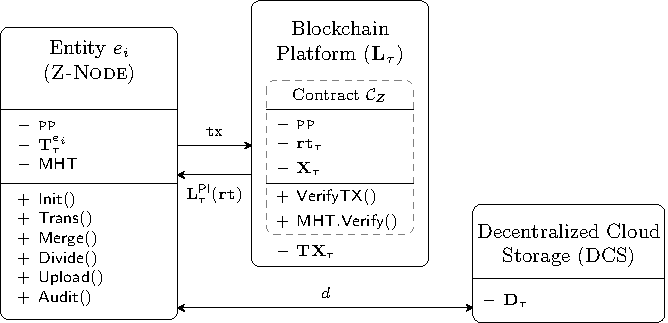
\includegraphics[width=0.8\linewidth]{Figures/Architecture}
    \caption[Primary components of the Zupply framework]{Primary components of the Zupply framework. In the figure, $\tau$ denotes time; \textsc{pp} represents public parameters; $\mathbf{T}_\tau^{e_i}$ denotes the set of \gls{aat}s associated with $e_i$; $\texttt{rt}_\tau$ is the root of the \textsf{MHT}; $\mathbf{X}_\tau$ is the set of \gls{aat}s that have reached their end-of-life (preventing re-transfer); \texttt{tx} denotes a transaction; $\mathbf{L}_\tau^\mathsf{PI}(\texttt{rt})$ is the proof-of-inclusion (PI) of $\texttt{rt}_\tau$ in the blockchain; $d$ denotes a data record; and $\mathbf{D}_\tau$ is the set of all such data records.}
    \label{fig:Zupply-Architecture}
\end{figure}

In the Zupply's \gls{dag} structure, data records are organized in sequences that can either split or merge. Except for the initial record, each one links back to its predecessor's \textsc{cid}. When sequences merge, they incorporate the \textsc{cid}s from previous records. Consequently, given any data record $d_n$, an auditor can trace back and retrieve all preceding records of $d_n$. This system allows any entity, such as a customer, to access a product's entire history up to that point by obtaining the most recent data record linked to the product, which could be uploaded by the last retailer in the chain. Given that the \textsc{cid} for each data record is derived from its multihash\footnote{Multihash is a self-identifying hash. It is a protocol designed to distinguish between the outputs of various established cryptographic hash functions \cite{multihash}.} \cite{Benet2014}, any modification to a record will invalidate the entire data sequence. 
% Also, each data record contains an encrypted section to ensure the confidentiality of sensitive information against public auditors. Appendix \ref{app:Data Encryption} suggests key management schemes to be employed in Zupply. 
Every data record comes with a \gls{zkp}, showing ownership of an \gls{aat} on the blockchain without revealing the owner's identity. Additionally, each record is digitally signed with a secret key, and the corresponding public key is a part of the \gls{aat}. 

In the initial stage of a supply chain (represented as a source vertex in a \gls{dag}), an \gls{aat} is created using the $\textsf{Init}$ algorithm, which is executed by the first entity. This token can then be passed along the supply chain to subsequent entities through \gls{aatot}, including three algorithms: $\textsf{Trans}$ for transferring the token, $\textsf{Merge}$ for combining two tokens before transferring, and $\textsf{Divide}$ for splitting a token into two tokens, which are then transferred. These processes, which employ \gls{zkp}s, not only ensure the token's continuous and secure progression through the supply chain but also preserve the unlinkability between entities. Entities within a supply chain can embed essential certificates into their data records to verify the product's originality to auditors. For instance, the initial data record could include a digital certificate of origin for a diamond, ensuring transparency and trust from the outset. However, subsequent entities responsible for transferring or storing the product can provide anonymous reports on conditions such as temperature, among others. These entities receive authorization to upload data from their predecessors, ensuring a secure and transparent chain of custody.

The Zupply Framework ensures that any entity uploading a data record has been authorized by its preceding entity. Therefore, it might be necessary for the first entity in a \gls{dag} to upload a certificate as a data record, allowing auditors to verify the source. This requirement remains indispensable in all \gls{scm} platforms, as customers check certificates issued by trusted certificate authorities, such as governments at the source or various steps of the supply chain. These certificates may or may not disclose the identity of the entities holding the certificates. In the initial stage of a \gls{dag}, the first \gls{aat} must be committed by an entity for its own use during the \textsf{Init} algorithm. While this process compromises the \gls{aat}'s anonymity, the authenticated data record will not reveal any information about the \gls{aat} itself. In contrast, the anonymity of owners for subsequently transferred tokens is maintained. This is because each \gls{aat} is committed by its preceding entity, ensuring the owner's anonymity. 


\subsection{Cryptographic Building Blocks}

Zupply utilizes the following cryptographic building blocks: 
\begin{enumerate}
    \item \textit{Statistically-hiding commitment} scheme (Definition \ref{def:Statistically-hiding commitment}) allows an entity to commit to their \gls{aat} $T$ by sending $\texttt{cm}:=\mathsf{COMM}_\rho(T)$ to the blockchain.

    \item \textit{Strongly-unforgeable digital signature} scheme (Definition \ref{def:Strongly-unforgeable digital signature}) is used for signing data records stored on \gls{dcs}.

    \item \textit{Symmetric-key encryption} scheme (Definition \ref{def:Symmetric-key encryption})  is used for encrypting the private part of data records.

    \item \textit{Zero-knowledge succinct non-interactive argument of knowledge} scheme (Definition \ref{def:zkSNARK Properties}) is used to ensure the authenticity of data records while preserving the anonymity of entities and unlinkability of \gls{aat} commitments.
\end{enumerate}


\subsection{Threat Model}

The adversary is driven by three primary motivations: the forgery or alteration of data records, the deanonymization of data uploaders, and the linking of collaborating entities. 

This adversary possesses the capability to access the blockchain, all data records stored on the \gls{dcs}, and observe all entities and their interactions with $\mathcal{C}_Z$. Zupply operates under the assumption that the adversary lacks possession of the product at each step of its lifecycle within the supply chain. This implies that they never hold an authentication token transferred from an authenticated entity. Therefore, any data reported by authorized entities, who are legitimately involved in the supply chain, is considered accurate. 

%A detailed discussion of the adversary's extensive assumptions, along with their objectives and potential attacks, is presented in Section \ref{sec:Attacker Model}.

\subsection{Security Goals}

The Zupply framework is designed as a trustless system for recording product histories, aiming to satisfy the following conditions:

\begin{enumerate}
\item The authenticity of data records, 
\item The integrity of data records,
\item The anonymity of data record uploaders and owners of transferred tokens,
\item The unlinkability among all entities collaborating within a supply chain.
\end{enumerate}


\subsection{Terms and Concepts in the Framework}
\label{sec:zupply-terms-and-concepts}
This section introduces the notations and symbols for data structures employed by Zupply. The symbol $\tau$ represents time and is also used to denote the state of each data structure. The superscript is for attribution, and the subscript is for indexing. For instance, \(T_i^{e_a}\) is the $i$th \gls{aat} which is attributed to or known by entity \(e_a\), while \(\texttt{tx}^{e_a}\) signifies that the transaction \(\texttt{tx}\) is published by \(e_a\) on the blockchain. Furthermore, to emphasize which entity runs a specific algorithm, the algorithm's name is presented as a superscript of the entity. For instance, if entity $e_a$ executes the algorithm \textsf{Init}, it is denoted as $e_a^\mathsf{Init}$.


\subsubsection{Entities}
\label{sec:Entities}
The set of all entities in Zupply is $\mathbf{E}_\tau = \{e_1, \dots, e_{|\mathbf{E}_\tau|}\}$. Each entity $e_i$, possesses a blockchain addresses denoted as $\text{BPAddr}^{e_i}$.  
This scheme operates without a central manager, placing all entities at an equal level of authority. Each entity runs the Zuppy Node (\textsc{Z-Node}).

\subsubsection{Anonymous Authentication Token (\gls{aat})}

For each \gls{aat} $T_i$  the keys $\text{SKsig}_{i}$ and $\text{PKsig}_{i}$ are generated using the key generation algorithm $\mathcal{K}_\mathsf{sig}$ based on a public key scheme, as defined in Definition~\ref{def:Strongly-unforgeable digital signature}.  Then, each \gls{aat} is represented as $T_i := (\Tilde{T}_i, \text{SKsig}_{i})$. Here $\Tilde{T}_i := (q_i, \text{PKsig}_{i}, \rho_i)$ denotes a partial \gls{aat}. Let $q_i \in \{0, 1\}^{N_q}$ keep track of the quantity of products, where ${N_q}$ is a  pre-determined security parameter which denotes the bit-length of quantity values in \glspl{aat}. It should be kept unchanged unless two supply chains are merged or one supply chain is divided into two sub supply chains. 

The owner of the \gls{aat} $T_i$ uses $\text{SKsig}_{i}$ to sign the data records uploaded by them. It is important not to confuse $\text{PKsig}_{i}$, which represents the public key associated with the token $T_i$, with the public keys related to the entity's $\text{BPAddr}$. 
Moreover, $\rho_i \in_R \{0, 1\}^{N_\rho}$, where ${N_\rho}$ is a  pre-determined security parameter which denotes the bit-length of $\rho$ values in \glspl{aat}, plays a crucial role in preventing the token's owner from re-transferring the \gls{aat} after transferring its ownership to the new owner(s). This is achieved by publishing the end-of-life (\gls{eol}) of the \gls{aat}, denoted as $\texttt{eol}_i = \mathcal{H}(\rho_i)$, on the blockchain. %Here, $\mathcal{H}$ represents a collision-resistant hash function. 
%\subsubsection{End of Life (\gls{eol})}
%In an \gls{aat}, $\rho_i \in_R \{0, 1\}^{N_\rho}$ prevents the owner of the \gls{aat} from re-transferring it after it has already been transferred by publishing the end-of-life (\gls{eol}), denoted as $\texttt{eol}_i = \mathcal{H}(\rho_i)$, on the blockchain.
$\mathbf{T}_\tau = \{T_1, \dots, T_{|\mathbf{T}_\tau|}\}$ denotes the time-ordered set of \gls{aat}s  and 
$\mathbf{X}_\tau = \{\texttt{eol}_1, \dots, \texttt{eol}_{|\mathbf{X}_\tau|}\}$ is the time-ordered set of published \gls{eol} of the obsoleted tokens. %We denote obsoleted token set at time $\tau$ as $\mathbf{O}_\tau$. Obsoleted tokens set is a subset of authentication tokens set $\mathbf{O}_\tau\subseteq \mathbf{T}_\tau$ for any $\tau$. 


\subsubsection{Commitment to Anonymous Authentication Token}
$\mathbf{C}_\tau = \{\texttt{cm}_1, \dots, \texttt{cm}_{|\mathbf{C}_\tau|}\}$ is the time-ordered set of commitments to $\mathbf{T}_\tau$. So, the corresponding commitment to  $T_i$ is denoted as $\texttt{cm}_i := \mathsf{COMM}_{\rho_i}(\Tilde{T_i})$. Figure \ref{fig:zupply-token} illustrates the diagram of committing to an \gls{aat}.




\begin{figure}
	\centering
	\includestandalone{Figures/TokenGenChart}
	\caption[Commitment to an Anonymous Authenticated Token]{The process of committing to an \gls{aat} and its corresponding \gls{eol}.}
	\label{fig:zupply-token}
\end{figure}


\subsubsection{Merkle Hash Tree}
Commitments to \gls{aat}s are stored on an $L$-layer Merkle hash tree ($|\mathbf{T}_\tau|<2^{L-1}$) denoted as $\mathsf{MHT}$ whose root is $\texttt{rt}_\tau$.
% The total number of anonymous authentication tokens is $|\mathbf{T}_\tau|<2^{L-1}$. 
Each leaf of $\mathsf{MHT}$ has an index number $ \mathsf{ind}\in [2^{L-1}]$ and $\mathsf{path}_\mathsf{ind}$ represents the Merkle proof corresponding to $\mathsf{ind}$. %The framework systematically populates the $\mathsf{MHT}$ following the order of the leaf indices. 
%A transition to the next state in the framework occurs if and only if one commitment is added to the $\mathsf{MHT}$. Consequently, $\texttt{rt}_\tau$ symbolizes the framework's state at time $\tau$. With this approach, we can define $\tau$ to be equivalent to the latest $\mathsf{ind}$, to which a commitment has been assigned. Moreover, $\mathsf{path}_\mathsf{ind}$ is the Merkle proof related to $\mathsf{ind}$.
$\mathsf{MHT}$ is a data structure that keeps the whole Merkle hash tree nodes and encompasses three algorithms: 
% $\mathsf{MHT}.\mathsf{Add}(\texttt{cm})$ is a stateful function which appends the new commitment to $\mathsf{MHT}$ and changes the \texttt{rt} accordingly. $\mathsf{MHT}.\mathsf{Verify}$ is a stateless function which verifies whether changing \texttt{rt} is consistent to the update of $\mathsf{MHT}$ (i.e., adding a new authentication token commitment to the tree): % The root of the Merkle tree (\texttt{rt}) is maintained $\mathsf{MHT}$ data structure. $\mathsf{MHT}$ has two methods:

\begin{enumerate} 

    \item $\mathsf{MHT}.\mathsf{Add}(\texttt{cm}) \rightarrow (\texttt{rt}^{\text{new}}, \mathsf{ind}, \mathsf{path}_\mathsf{ind})$. Given a new \texttt{cm},  the algorithm adds \texttt{cm} to the $\mathsf{MHT}$ and outputs the new Merkle root $\texttt{rt}^{\text{new}}$, the index of the new commitment ($\mathsf{ind}$), and $\mathsf{path}_\mathsf{ind}$.

    % \item $\mathsf{MHT}.\mathsf{Verify}(\texttt{cm}, \mathsf{path}) \rightarrow \{0, 1\}$. Given a commitment \texttt{cm} and Merkle path ($\mathsf{path}$),  $\mathsf{MHT}.\mathsf{Verify}$ outputs $1$ if \texttt{cm} is in $\mathsf{MHT}$, otherwise returns $0$.

    \item $\mathsf{MHT}.\mathsf{Verify}(\texttt{rt}_{\tau-1}, \texttt{rt}_{\tau}, \texttt{cm}, \mathsf{ind}, \mathsf{path}_\mathsf{ind})$ $ \rightarrow $ $\{0, 1\}$. Given the previous and the new root of $\mathsf{MHT}$ before and after assigning \texttt{cm} to the tree at  $\mathsf{ind}$, with corresponding $\mathsf{path}_\mathsf{ind}$, this algorithms verifies whether $\texttt{rt}_{\tau}$ is computed correctly.

    \item $\mathsf{MHT}.\mathsf{Search}(\texttt{cm}_i)$ $ \rightarrow $ $(\mathsf{ind}_i, \mathsf{path}_{\mathsf{ind}_i})$. Given  $\texttt{cm}_i$, $\mathsf{MHT}.\mathsf{Search}$ returns the index of  $\texttt{cm}_i$ ($\mathsf{ind}_i$), and the corresponding $\mathsf{path}_{\mathsf{ind}_i}$.
    
    % the previous and the new root of $\mathsf{MHT}$ before and after assigning \texttt{cm} to the leaf at the latest index  $\mathsf{ind} = \tau$ and the corresponding Merkle proof $\mathsf{path}_\mathsf{ind}$, this algorithms verifies whether $\texttt{rt}_{\tau}$ is consistent to $\texttt{rt}$ after this update or not.
\end{enumerate}

$\mathsf{MHT}.\mathsf{Add}()$ and $\mathsf{MHT}.\mathsf{Search}()$ are stateful, having direct access to the \textsf{MHT} data structure. In contrast, $\mathsf{MHT}.\mathsf{Verify}()$ does not. This algorithm is implemented within the smart contract, which does not store the \textsf{MHT}. %Detailed explanation of this algorithm is provided in Section \ref{sec:MerkleTreeStructure}.

\subsubsection{Blockchain Platform Ledger}
We can model the blockchain as an immutable, public, decentralized ledger, denoted as $\mathbf{L}_\tau$, on which the Zupply smart contract, $\mathcal{C}_Z$, is deployed.  $\mathcal{C}_Z$ maintains $\texttt{rt}_\tau$, and $\mathbf{X}_\tau$. The commitments in $\mathbf{C}_\tau$ are uploaded to the blockchain via transactions that invoke $\mathcal{C}_Z$. Consequently, $\mathbf{L}_\tau$ records all transactions associated with the Zupply framework (discussed below), along with other unrelated transactions on the blockchain platform.

Wherever data records are concerned, the protocol employs the \textit{proof-of-inclusion (\gls{pi})} mechanism provided by the blockchain to prove the correctness of the value $\texttt{rt}_\tau$ used in off-chain proofs. The PI of $\texttt{rt}_\tau$ in ledger $\mathbf{L}_\tau$ at time $\tau$ is represented as $\mathbf{L}_\tau^\mathsf{PI}(\texttt{rt})$. This proof ensures that the auditors can  verify  $\texttt{rt}$ employed for off-chain authentication.  

\subsubsection{Transactions}
Each transaction  $\texttt{tx}$ $\in$ $\{ \texttt{tx}_\textsf{Init},$ $\texttt{tx}_\textsf{Trans},$ $\texttt{tx}_\textsf{Merge},$ $\texttt{tx}_\textsf{Div} \}$ invokes a specific function in $\mathcal{C}_Z$. Each $\texttt{tx}$ contains one or two \texttt{cm}s, and whenever it finalizes on the blockchain,  its corresponding \texttt{cm}s are added to \textsf{MHT} locally and updates $\texttt{rt}_\tau$  on the blockchain. For a transactions that transfers the ownership of \gls{aat}(s), $\texttt{tx} \in \{$$\texttt{tx}_\textsf{Trans}$, $\texttt{tx}_\textsf{Merge}$, $\texttt{tx}_\textsf{Div}$ $\}$, the transaction contains the \gls{eol} of \gls{aat}(s) whose commitment(s) are stored on $\mathsf{MHT}$, and a \gls{zkp} of owning them. These proofs are denoted as $\pi_\mathbbm{x} \in \{\pi_\textsf{Trans}, \pi_\textsf{Merge}, \pi_\textsf{Div} \}$. The \gls{eol} should not be included in $\mathbf{X}_\tau$ prior to issuing the transaction. Only after the transaction is finalized by $\mathcal{C}_Z$, the smart contract updates $\mathbf{X}_\tau$ by adding the \gls{eol} to it.
% The transactions also contain the \textsf{BP} address of the transaction issuer, denoted as $\mathsf{BPAddr}^{e_i}$, which belongs to the entity $e_i$. 
The time-ordered set of transactions on blockchain is denoted as $\mathbf{TX}_\tau = \{\texttt{tx}_1, \dots, \texttt{tx}_{|\mathbf{TX}_\tau|}\}$.


% Zupply protocol employs an immutable public decentralized ledger denoted as $\mathbf{L}_\tau$ which keeps all the authentication token commitments ($\mathbf{C}_\tau$). The authentication token commitments are uploaded to the ledger via one the transactions $\texttt{tx}$ $\in$ $\{ \texttt{tx}_\textsf{Init}$$,$ $\texttt{tx}_\textsf{Trans}$$,$ $\texttt{tx}_\textsf{Merge}$$,$ $\texttt{tx}_\textsf{Div} \}$ which calls the Zupply smart contract $\mathcal{C}_Z$ deployed on the ledger. The smart contract maintains the value of the Merkle tree root $\texttt{rt}$. Wherever, specifically on data records, the protocol needs to prove the correctness of the value $\texttt{rt}$ on blockchain, it employs the \textit{proof-of-inclusion} provided by the blockchain platform. For example, Ethereum uses Merkle Patricia Trie \cite{PatriciaTree}. In this paper the poof-of-inclusion of $\texttt{rt}$ in ledger $\mathbf{L}_\tau$ is denoted as $\mathbf{L}_\tau(\texttt{rt})$.

\begin{figure}
	\centering
	\includestandalone[width=0.8\linewidth]{Figures/DataChain}
	% \includestandalone{./Figures/TokenGenChart}
	\caption[Data records in the Zupply framework]{Data records create a DAG structured data. $d_n$ represents the data record after two data sequences merges in the DAG.}
	\label{fig:zupply-datachain}
\end{figure}

\subsubsection{Data Records}
The time-ordered set of data records is denoted as $\mathbf{D}_\tau = \{d_1, \dots, d_{|\mathbf{D}_\tau|}\}$. Data records are stored on a \gls{dcs}. 
The \gls{cid} of a data record $d_n$ in the \gls{dcs} is denoted as $\textsc{cid}_n$.
The set of all \gls{cid}s is $\mathbf{CID}_\tau = \{\textsc{cid}_1, \dots, \textsc{cid}_{|\mathbf{CID}_\tau|}\}$. 
$\mathsf{DCS}(\textsc{cid}_n) \rightarrow d_n$ denotes a query to the \gls{dcs} to get the data record corresponded  \textsc{cid}.
% We can query the DCS to get the data record corresponded to each \textsc{cid}. The query is denoted as  $\mathsf{DCS}(\textsc{cid}_n) \rightarrow d_n$. %since each data record is corresponded to a content identifier, $|\mathbf{D}_\tau| = |\mathbf{CID}_\tau|$.
% Each data record $d_n$ is linked to two predecessor data records $d_p$ and $d_q$, where $p,q < n$. 
Each data record $d_n$ contains references to its predecessor, $d_p$ and $d_q$, where $p,q < n$, in the array $d_n.\mathsf{pred}$ if applicable. Specifically, $d_n.\mathsf{pred}[b] \in \mathbf{CID}_\tau$ for ${b = 0, 1}$; although one or both entries of the array may be $\emptyset$.
A data record $d_n$ contains public data $d_{n, \mathsf{pub}}$ which is stored as plain-text, and private data $d_{n, \mathsf{pri}}$ which is stored as cipher-text $c_n = \mathcal{E}_\mathsf{sym}(\textsc{k}_n, d_{n, \mathsf{pri}})$. Zupply may incorporate the forward secrecy scheme outlined in Mesh \cite{altawy2019mesh} to determine $\textsc{k}_n$ (Appendix \ref{app:Data Encryption}). $d_n$ also includes a \gls{zkp} $\pi_\textsf{Auth}$ of owning $T_i$ such that its corresponding $\texttt{cm}_i$ is in \textsf{MHT}.  The public input to this proof is denoted as $x_\texttt{Auth}$. Each $T_i$, can be used more than once to prove authenticity.
Also, the data record $d_n$ includes $\sigma_n = \mathcal{S}_\mathsf{sig}(\text{SKsig}_i, d_n)$, where $\text{SKsig}_i$ is the secret key associated with $\text{PKsig}_{i}$ in $T_i$. Consequently, $d_n$ is denoted as the following tuple and illustrated in Figure \ref{fig:zupply-datachain}:
\begin{align*}
    d_n  := & \left( d_{n, \mathsf{pub}}, c_n, \mathsf{pred}=\{\textsc{cid}_p, \textsc{cid}_q\}, \mathsf{tags}=\{\texttt{Tag}_p, \texttt{Tag}_q\}, \right. \\ 
    & \left. \pi_\textsf{Auth}, x_\textsf{Auth}=\{\texttt{rt}_\tau, \text{PKsig}_{i}\}, \mathbf{L}_\tau^\mathsf{PI}(\texttt{rt}_\tau) \right),
\end{align*}
where the digital signature $\sigma_n$  is uploaded together with the data  $d_n$ and the data ownership transfer tags (\textsf{tags}) are explained in the following.

\subsubsection{Data Ownership Transfer Tag} 
\label{sec:Data ownership transfer tag}

% The protocol enforces using data ownership transfer tag denoted as $\texttt{Tag}$ 
When two consecutive data records $d_{n-1}, d_n$ in a data sequence uses different secret keys for signing the data records. Namely, $\sigma_{n-1} = \mathcal{S}_\mathsf{sig}(\text{SKsig}_i, d_{n-1})$ and $\sigma_n = \mathcal{S}_\mathsf{sig}(\text{SKsig}_j, d_n)$. In this scenario, the later data record ($d_n$) has to include the $\texttt{Tag}_i = \mathcal{S}_\mathsf{sig}(\text{SKsig}_i, \text{PKsig}_j)$ created by the owner of the former data record ($d_{n-1}$). Data ownership transfer tags are created and used in \gls{aatot} presented in Section \ref{sec:Ownership Transfer}.


\subsubsection{Directed Acyclic Graph}
Given that each data record can reference its predecessor, they collectively form a DAG. Consequently, we define three key concepts integral to our DAG data structure:
\begin{enumerate}
    \item \textit{Init data ($d_{n, \mathsf{Init}}$)}: Any data record $d_n$ which does not have any predecessor, i.e., $d_n.\mathsf{pred}[b] = \emptyset$ for both ${b \in \{0, 1\}}$. %, initiates a new DAG. The data record $d_i$ is an \textit{Init} data record and denoted as $d_{i, \mathsf{Init}}$.

    \item \textit{Data Sequence ($S_k$)}: $S_k$ is a sequence of data records where each data record has one and only one predecessor. The first data record in $S_k$ can have zero, one, or two predecessors. %Namely, \textit{Data Sequence} $S_k$ is a time-ordered set of data records denoted as $S_k = \{d_{i_1}, \dots, d_{i_m}\}$ where $\forall n \in [2, m]$,  $d_{i_n}.\mathsf{pred}[0] = \textsc{cid}_{i_{n-1}}$, $d_{i_n}.\mathsf{pred}[1] =\emptyset$. 

    \item \textit{Progressive Data Sequence ($\hat{S}_k$)}: is a data sequence denoted as $\hat{S}_k = \{d_{i_1}, \dots, d_{i_m}\}$, where data record $d_{i_m}$ is the most recent, and it's ensured that no subsequent data record references $d_{i_m}$.

    % \item \textit{Forking Attack}: The potential attack to a data sequence is forking attack. For a data sequence $S_k$ such that $d_n \in S_k$, the adversary uploads a data 
\end{enumerate}






% \begin{remark} [\textsf{MHT} State-Related Algorithms]

% \end{remark}

\begin{remark} [\gls{aat} Public Key]
In the $\pi_\textsf{Auth}$, $\text{PKsig}$ is used as a public input. $\pi_\textsf{Auth}$ is then published off-chain on data records. However, for proofs directly published on the blockchain ($\pi_\textsf{Trans}$, $\pi_\textsf{Merge}$, and $\pi_\textsf{Div}$), $\text{PKsig}$ is treated as a private input. Also, the $\text{PKsig}$ is never published on blockchain. 
\end{remark}


\begin{definition}[Valid \gls{aat}]
	\label{def:Valid Authentication Token}
	$T_{i_2}$ is a valid \gls{aat} for authenticating a data record $d_{n_2}$ if and only if
	the $\texttt{cm}_{i_2} := \mathsf{COMM}_{\rho_{i_2}}(T_{i_2})$ is included in \textsf{MHT}.
\end{definition}


\begin{definition}[Authenticated Data]
	\label{def:Authenticated Data}
	A data record $d_{n}$ is an authenticated data if and only if $d_{n}$ contains
	\begin{enumerate}
		\item  a valid zero-knowledge proof of ($\pi_\texttt{Auth}$) of owning a \textit{valid \gls{aat}} $T_{i}$ (Definition \ref{def:Valid Authentication Token}).
		\item a valid signature $\sigma$ is created using the secret key $\text{SKsig}_{i}$, ensuring that both it and its corresponding public key $\text{PKsig}_{i}$ are included in $T_{i}$.
		\item valid tag(s) if and only if the predecessor data record is signed by different key(s) and $d_{n}.\text{pred} \neq \emptyset$
	\end{enumerate}
\end{definition}

\begin{definition}[Valid Transaction]
	\label{def:Valid Transaction}
	A transaction $\texttt{tx} $ $ \in $ $ \{ \texttt{tx}_\textsf{Init}, $ $ \texttt{tx}_\textsf{Trans}, $ $ \texttt{tx}_\textsf{Merge}, $ $ \texttt{tx}_\textsf{Div} \}$ is a valid transaction if and only if
	\begin{enumerate}
		\item $\mathsf{MHT}.\mathsf{Verify}(\texttt{rt}_{\tau}, \texttt{rt}^\text{new}, \texttt{cm}, \mathsf{ind}, \mathsf{path}_\mathsf{ind}) = 1$, where The root of \textsf{MHT} was $\texttt{rt}_{\tau}$ before $\texttt{tx}$. For $\textsf{Div}$ transaction (i.e., $\texttt{tx}= \texttt{tx}_\textsf{Div}$) the transition of the root is examined in two rounds of running $\mathsf{MHT}.\mathsf{Verify}$ algorithm: $\texttt{rt}_\tau \rightarrow \texttt{rt}^\text{new}_1 \rightarrow \texttt{rt}^\text{new}_2$. 
		
		
		\item $\texttt{eol} \notin  \mathbf{X}_\tau$. Where $\texttt{tx}_\mathsf{Trans}$ and $\texttt{tx}_\mathsf{Div}$ contain one and $\texttt{tx}_\mathsf{Merge}$ contains two \texttt{eol}s. This value represents the \gls{aat} that is expired during the owner transferring algorithms.
		
		\item $\mathsf{Verify}(\text{vk}_\mathbbm{x}, x_\mathbbm{x}, \pi_\mathbbm{x}) = 1$ for $\mathbbm{x} \in \{\mathsf{Trans}$, $\mathsf{Merge}$, $\mathsf{Div} \}$
		
	\end{enumerate}
\end{definition}




\subsection{NP Statements}
\label{sec:Zero-knowledge Proofs}
This section presents the \gls{np}-statements related to \gls{zkp}s employed in Zupply. 


\subsubsection{Authenticity proof ($\pi_\textsf{Auth}$)}
Whenever an entity wants to upload a data record on \gls{dcs}, the entity (prover) proves they own a commitment \texttt{cm} in the \textsf{MHT}. The \gls{np} problems associated with this proof are explained as follows:

    
\begin{itemize}

    \item $\texttt{cm}_i =\mathsf{COMM}_{\rho_i}(\Tilde{T}_i)$
	\item $\texttt{path}_i$ is a valid path from leaf  $\texttt{cm}_i$ to root $\texttt{rt}_\tau$.
\end{itemize}

Where $\Tilde{T}_i = (q_i, \text{PKsig}_i, \rho_i)$. To prove that the used \texttt{rt} is a valid value stored on $\mathcal{C}_Z$, the entity provides the \gls{pi} $\mathbf{L}_\tau^\mathsf{PI}(\texttt{rt})$.



\subsubsection{Transferability proof ($\pi_\textsf{Trans}$)}

When an entity wishes to transfer the ownership of an \gls{aat} ($T_{i_1}$), it (as the prover) proves that the newly minted $\Tilde{T}_{i_2}$ maintains the same product quantity as $T_{i_1}$ (i.e., $q_{i_1} = q_{i_2}$), without disclosing details about $T_{i_1}$ and $\Tilde{T}_{i_2}$. Moreover,  $\texttt{cm}_{i_1}$ is kept confidential. In addition, the entity proves that the published $\texttt{eol}_{i_1}$ is equal to $\mathcal{H}(\rho_{i_1})$, while keeping $\rho_{i_1}$ secret. The \gls{np} problems associated with this proof are explained as follows:

\begin{itemize}
	\item $\texttt{eol}_{i_1} = \mathcal{H}(\rho_{i_1} )$
	\item $\texttt{cm}_{i_1} = \mathsf{COMM}_{\rho_{i_1}}(\Tilde{T}_{i_1})$
	\item $\texttt{path}_{{i_1}}$ is a valid path from leaf  $\texttt{cm}_{\texttt{cm}_{i_1}}$ to root $\texttt{rt}_\tau$
	\item $\texttt{cm}_{i_2} = \mathsf{COMM}_{\rho_{i_2}}(\Tilde{T}_{i_2})$
	\item $q_{i_1} = q_{i_2} $
\end{itemize}
Where  $\Tilde{T}_{i_1} = (q_{i_1}, \text{PKsig}_{i_1}, \rho_{i_1})$, $\Tilde{T}_{i_2} = (q_{i_2}, \text{PKsig}_{i_2}, \rho_{i_2})$, and $x_\mathsf{Trans} = (\texttt{eol}_{i_1}, \texttt{cm}_{i_2}, \texttt{rt}_\tau)$ denotes the public inputs.

\subsubsection{Mergeability proof ($\pi_\textsf{Merge}$)}
An entity may merge two \gls{aat}s $T_{i_1}$ and $T_{i_2}$ to create $T_{i_3}$. The entity proves that the quantity in $T_{i_3}$ is the same as the summation of quantities in $T_{i_1}$ and $T_{i_2}$ (i.e., $q_{i_1} + q_{i_2} = q_{i_3}$).  The \gls{zkp} $\pi_\mathsf{Merge}$ follows the same approach as $\pi_\mathsf{Trans}$. The \gls{np} problems associated with this proof are explained as follows:
\begin{itemize}
    \item $\texttt{eol}_{i_1} = \mathcal{H}(\rho_{i_1} )$ and $\texttt{eol}_{i_2} = \mathcal{H}(\rho_{i_2} )$
	\item $\texttt{cm}_{i_1} = \mathsf{COMM}_{\rho_{i_1}}(\Tilde{T}_{i_1})$, $\texttt{cm}_{i_2} = \mathsf{COMM}_{\rho_{i_2}}(\Tilde{T}_{i_2})$

	\item $\texttt{path}_{{i_1}}$ and $\texttt{path}_{{i_2}}$  are valid paths respectively from leaf  $\texttt{cm}_{\texttt{cm}_{i_1}}$  and 
      $\texttt{cm}_{\texttt{cm}_{i_2}}$ to root $\texttt{rt}_\tau$.

    \item $\texttt{cm}_{i_3} = \mathsf{COMM}_{\rho_{i_3}}(\Tilde{T}_{i_3})$
	\item $q_{i_1} + q_{i_2} = q_{i_3} $
    
\end{itemize}
Where  $\Tilde{T}_{i_1} = (q_{i_1}, \text{PKsig}_{i_1}, \rho_{i_1})$, $\Tilde{T}_{i_2} = (q_{i_2}, \text{PKsig}_{i_2}, \rho_{i_2})$ and $\Tilde{T}_{i_3} = (q_{i_3}, \text{PKsig}_{i_3}, \rho_{i_3})$.
The public input to the proof is denoted as $x_\mathsf{Merge} = (\texttt{eol}_{i_{1,2}}, \texttt{cm}_{i_3}, \texttt{rt}_\tau)$.


\subsubsection{Divisibility proof ($\pi_\textsf{Div}$)}
An entity can divide an \gls{aat} $T_{i_1}$ into two new ${T}_{i_2}$ and ${T}_{i_3}$. The approach of creating \gls{zkp} $\pi_\textsf{Div}$ follows the same approaches in $\pi_\textsf{Trans}$ and $\pi_\textsf{Merge}$. The \gls{np} problems associated with this proof are explained as follows:

\begin{itemize}
    \item $\texttt{eol}_{i_1} = \mathcal{H}(\rho_{i_1} )$
	\item $\texttt{cm}_{i_1} = \mathsf{COMM}_{\rho_{i_1}}(\Tilde{T}_{i_1})$
	\item $\texttt{path}_{{i_1}}$ is a valid path from leaf  $\texttt{cm}_{\texttt{cm}_{i_1}}$ to root $\texttt{rt}_\tau$


    \item $\texttt{cm}_{i_2} = \mathsf{COMM}_{\rho_{i_2}}(\Tilde{T}_{i_2})$ and $\texttt{cm}_{i_3} = \mathsf{COMM}_{\rho_{i_3}}(\Tilde{T}_{i_3})$
	\item $q_{i_1} = q_{i_2} + q_{i_3}$
    
\end{itemize}
Where  $\Tilde{T}_{i_1} = (q_{i_1}, \text{PKsig}_{i_1}, \rho_{i_1})$, $\Tilde{T}_{i_2} = (q_{i_2}, \text{PKsig}_{i_2}, \rho_{i_2})$ and $\Tilde{T}_{i_3} = (q_{i_3}, \text{PKsig}_{i_3}, \rho_{i_3})$. The public input is denoted as $x_\mathsf{Div} =\big(\texttt{eol}_{i_1}, \texttt{cm}_{i_{2,3}}, \texttt{rt}_\tau \big)$.

\section{Zupply Algorithms and Protocols}
\label{sec:Zupply Algorithms}
The Zupply framework comprises a set of  algorithms and protocols detailed in Sections \ref{sec:Zupply-Algorithms} and \ref{sec:Zupply-Protocols}, respectively.

\begin{definition}[Zupply Framework]
\label{def:Zupply Framework}
Zupply framework $\Pi$ Consists of a tuple of polynomial-time algorithms and protocols $\Pi = $ ($\textsf{Setup}$, $\textsf{Init}$,  $\textsf{Trans}$, $\textsf{Merge}$, $\textsf{Divide}$, $\textsf{Upload}$, $\textsf{VerifyTX}$, $\textsf{Audit}$; $\textsf{OT-Protocol}$, $\textsf{MHT-Protocol}$).
\end{definition}



\subsection{Algorithms} \label{sec:Zupply-Algorithms}%
% Using security parameter $\lambda$, we define Zupply Scheme. // explain $i$
All algorithms have read-only access to $\mathbf{TX}\tau$, $\mathbf{C}\tau$, \textsf{MHT}, $\mathbf{X}\tau$, and $\mathbf{D}\tau$ (accessible via \textsf{DCS} queries). The smart contract is responsible for updating $\mathbf{TX}\tau$, $\mathbf{C}\tau$, $\mathbf{X}_\tau$, and the root of \textsf{MHT} when the \textsf{VerifyTX} algorithm outputs 1.

\subsubsection{\textsf{Setup} ($1^{\lambda}$) $\rightarrow$ $\textsc{pp}$}
Given a security parameter $\lambda$, \textsf{Setup} generates a set of global public parameters, denoted as \textsc{pp}. The specific implementation of \textsf{Setup} depends on the \gls{zksnark} algorithm in use: it may require a trusted party, or it may rely on a transparent (public) setup. The resulting \textsc{pp} is made publicly available. The pseudocode for \textsf{Setup} is provided in Algorithm~\ref{alg:Setup}.

%%%%%%%%%%%%%%%%%%%%%%%%%% Setup %%%%%%%%%%%%%%%%%%%%%%%%%%
\begin{algorithm}[h]
\caption{\textsf{Setup} ($1^{\lambda}$) $\rightarrow$ $\textsc{pp}$ }\label{alg:Setup}
\begin{algorithmic}

\State $(\text{pk}_\texttt{Auth}, \text{vk}_\texttt{Auth}) \leftarrow \textsf{KeyGen}(1^{\lambda}, \mathsf{Auth})$ 

\State $(\text{pk}_\textsf{Trans}, \text{vk}_\textsf{Trans}) \leftarrow \textsf{KeyGen}(1^{\lambda}, \mathsf{Trans})$ 

\State $(\text{pk}_\textsf{Merge}, \text{vk}_\textsf{Merge}) \leftarrow \textsf{KeyGen}(1^{\lambda}, \mathsf{Merge})$ 

\State $(\text{pk}_\textsf{Div}, \text{vk}_\textsf{Div}) \leftarrow \textsf{KeyGen}(1^{\lambda}, \mathsf{Divide})$ 

\State $\textsc{pp}_\mathsf{sig} \leftarrow \mathcal{G}_\mathsf{sig}(1^{\lambda})$


\State $\textsc{pp}$ $\leftarrow$ $($$\text{pk}_\texttt{Auth}$, $\text{vk}_\texttt{Auth}$, $\text{pk}_\textsf{Trans}$, $\text{vk}_\textsf{Trans}$, $\text{pk}_\textsf{Merge}$, $\text{vk}_\textsf{Merge}$, $\text{pk}_\texttt{Div}$, $\text{vk}_\texttt{Div}$, $\textsc{pp}_\mathsf{sig}$ $)$

\State \Return $\textsc{pp}$

\end{algorithmic}
\end{algorithm}
% ###########################################


\subsubsection{\textsf{Init} ($\textsc{pp}$, $q_{i_1}$) $\rightarrow$ ($\texttt{tx}_{\textsf{Init}}$, $T_{i_1}$) }
Initiates a \gls{dag}. The algorithm gets $q_{i_1}$, which will be maintained in the \gls{dag}. It creates a new token $T_{i_1}$, commits to it, and sends the commitment via
 \[
 \texttt{tx}_{\mathsf{Init}} := (\texttt{cm}_{i_1}, \texttt{rt}^{\text{new}}, \mathsf{ind}_{i_1}, \mathsf{path}_{\mathsf{ind}_{i_1}})
 \]
 to the blockchain. The pseudocode for \textsf{Init} is provided in Algorithm~\ref{alg:Init} is provided in Algorithm~\ref{alg:trans} in Appendix \ref{a_ch:zupply_algorithms}.



\subsubsection{\textsf{Trans} (\textsc{pp}, $T_{i_1}$,  $\text{PKsig}_{i_2}$) $\rightarrow$ ($\texttt{tx}_{\textsf{Trans}}$, $\Tilde{T}_{i_2}$, $\texttt{Tag}$)}

This algorithm takes an existing \gls{aat} $T_{i_1}$ and renders it obsolete by publishing its associated \gls{eol} on the blockchain. Specifically, it computes $\texttt{eol}_{i_1} := \mathcal{H}(\rho_{i_1})$, where $\rho_{i_1}$ is a secret contained in $T_{i_1}$, and includes this value in the resulting transaction $\texttt{tx}_{\textsf{Trans}}$.
Subsequently, the algorithm constructs a new partial \gls{aat}, denoted $\Tilde{T}_{i_2}$, by sampling a fresh random value $\rho_{i_2}$ and assigning it the same quantity as in $T_{i_1}$. The public key $\text{PKsig}_{i_2}$ is used to bind the new token to its intended recipient, in accordance with the \textsf{OT-Protocol} described in Section~\ref{sec:Ownership Transfer}. The algorithm commits to $\Tilde{T}_{i_2}$ and includes the resulting commitment in the transaction.
The transaction also includes a \gls{zkp} demonstrating:
(1)  knowledge of $T_{i_1}$ whose commitment is included in the \textsf{MHT}, without revealing the commitment itself,
(2) consistency of this committment with the published $\texttt{eol}_{i_1}$,
(3) knowledge of the preimage of the new commitment ($\texttt{cm}_{i_2}$) to $\Tilde{T}_{i_2}$, and
(4) equality of the quantity values in $T_{i_1}$ and $\Tilde{T}_{i_2}$.
Accordingly, the contents of the transaction $\texttt{tx}_{\textsf{Trans}}$ are defined as:
\[
\texttt{tx}_{\textsf{Trans}} := \big(\pi_{\textsf{Trans}}, x_{\textsf{Trans}}, \texttt{eol}_{i_1}, \texttt{cm}_{i_2}, \texttt{rt}^{\text{new}}, \mathsf{ind}_{i_2}, \mathsf{path}_{\mathsf{ind}_{i_2}} \big)
\]
where 
\[
x_\textsf{Trans} := \big(\texttt{eol}_{i_1}, \texttt{cm}_{i_2}, \texttt{rt}_\tau \big)
\]
denotes the public inputs to the \gls{zkp}, $\texttt{rt}^{\text{new}}$ is the updated root of the \textsf{MHT} after inserting the new commitment $\texttt{cm}_{i_2}$, and $\mathsf{ind}_{i_2}$ with $\mathsf{path}_{\mathsf{ind}{i_2}}$ represent the index and Merkle proof of the new commitment.
Finally, the algorithm outputs a $\texttt{Tag}$, which enables the new \gls{aat} owner to continue the data sequence, ensuring continuity with the most recent data record generated using $T_{i_1}$. The pseudocode for \textsf{Trans} is provided in Algorithm~\ref{alg:trans} in Appendix~\ref{a_ch:zupply_algorithms}.




\subsubsection{\textsf{Merge} (\textsc{pp}, $T_{i_{1}}$, $T_{i_{2}}$,  $\text{PKsig}_{i_3}$) $\rightarrow$ ($\texttt{tx}_{\textsf{Merge}}$, $\Tilde{T}_{i_3}$, $\texttt{Tag}_{i_{1}}$, $\texttt{Tag}_{i_{2}}$)}

The \textsf{Merge} algorithm follows a similar approach to the \textsf{Trans} algorithm. In this procedure, two \glspl{aat}, $T_{i_1}$ and $T_{i_2}$, are rendered obsolete, and their corresponding \glspl{eol}, $\texttt{eol}_{i_{1}}$ and $\texttt{eol}_{i_{2}}$, are published to the blockchain via $\texttt{tx}_{\textsf{Merge}}$. A new partial token, $\Tilde{T}_{i_3}$, is created using the input public key $\text{PKsig}_{i_3}$, sampling a random value $\rho_{i_2}$, and a quantity value set to the sum of the quantity values in $T_{i_1}$ and $T_{i_2}$.
The transaction also includes a commitment to the new \gls{aat}, denoted by $\texttt{cm}_{i_3}$, along with a \gls{zkp} that proves the following statements without revealing the underlying values: (1) knowledge of $T_{i_1}$ and $T_{i_2}$ whose commitments are included in the \textsf{MHT}, (2)  consistency of these commitments with the published $\texttt{eol}_{i_{1}}$ and $\texttt{eol}_{i_{2}}$, (3) the knowledge of $\Tilde{T}{i_3}$ in the new commitment $\texttt{cm}_{i_3}$ to $\Tilde{T}_{i_3}$, and (4) that the quantity in $\Tilde{T}_{i_3}$ equals the sum of the quantities in $T_{i_1}$ and $T_{i_2}$.  Accordingly, the transaction $\texttt{tx}_{\textsf{Merge}}$ is defined as:
\[
\texttt{tx}_\mathsf{Merge} :=(\pi_{\mathsf{Merge}}, x_\mathsf{Merge}, \texttt{eol}_{i_{1}}, \texttt{eol}_{i_{2}},  \texttt{cm}_{i_3}, \texttt{rt}^{\text{new}}, \mathsf{ind}_{i_3}, \mathsf{path}_{\mathsf{ind}_{i_3}}),
\]
where
\[
x_\mathsf{Merge} = (\texttt{eol}_{i_{1}}, \texttt{eol}_{i_{2}} \texttt{cm}_{i_3}, \texttt{rt}_\tau)
\]
denotes the public inputs to the \gls{zkp}. Here, $\texttt{rt}_1^{\text{new}}$ is the updated root of the \textsf{MHT} after inserting the first new commitment $\texttt{cm}_{i_2}$, and $\texttt{rt}_2^{\text{new}}$ is the root after inserting the second new commitment $\texttt{cm}_{i_3}$. Accordingly, $\mathsf{ind}_{i_2}$ with its corresponding Merkle path $\mathsf{path}_{\mathsf{ind}_{i_2}}$, and $\mathsf{ind}_{i_3}$ with $\mathsf{path}_{\mathsf{ind}_{i_3}}$, represent the indices and Merkle proofs for the first and second new commitments, respectively.
The \textsf{Merge} algorithm also outputs two data ownership transfer tags, $\texttt{Tag}_{i_{1}}$ and $\texttt{Tag}_{i_{2}}$, which are used together in a new data record to ensure continuity with the two most recent data records generated by the \glspl{aat} $T_{i_1}$ and $T_{i_2}$ and merging those sequences. The pseudocode for the \textsf{Merge} algorithm is provided in Algorithm~\ref{alg:merge} in Appendix~\ref{a_ch:zupply_algorithms}.

%Obsoletes $T_{i_1}$, $T_{i_2}$ and generates $\Tilde{T}_{i_3}$ ($q_{i_3} = q_{i_1} + q_{i_2}$).  $T_{i_1}$, $T_{i_2}$, $\Tilde{T}_{i_3}$, $\texttt{cm}_{i_1}$, and $\texttt{cm}_{i_2}$ are not disclosed. $\texttt{tx}_\mathsf{Merge} $:$=(\pi_{\mathsf{Merge}}, x_\mathsf{Merge}, \texttt{eol}_{i_{1,2}},  \texttt{cm}_{i_3}, \texttt{rt}^{\text{new}}, \mathsf{ind}_{i_3}, \mathsf{path}_{\mathsf{ind}_{i_3}} )$,
% where $x_\mathsf{Merge} = (\texttt{eol}_{i_{1,2}}, \texttt{cm}_{i_3}, \texttt{rt}_\tau)$.



\subsubsection{\textsf{Divide} ($\textsc{pp}$, $T_{i_1}$,  $\text{PKsig}_{i_{2}}$, $\text{PKsig}_{i_{3}}$, $q_{i_{2}}$, $q_{i_{3}}$) $\rightarrow$ ($\texttt{tx}_{\textsf{Div}}$, $\Tilde{T}_{i_{2}}$, $\Tilde{T}_{i_{3}}$, $\texttt{Tag}_{i_{2}}$, $\texttt{Tag}_{i_{3}}$)}

The \textsf{Divide} algorithm is the inverse of the \textsf{Merge} algorithm. It takes a single \gls{aat}, $T_{i_1}$, as input and creates two new partial \glspl{aat}, denoted $\Tilde{T}_{i_2}$ and $\Tilde{T}_{i_3}$. These are generated using the provided public keys $\text{PKsig}_{i_2}$ and $\text{PKsig}_{i_3}$, sampled random values $\rho_{i_2}$ and $\rho_{i_3}$, and quantity values $q_{i_2}$ and $q_{i_3}$, such that the sum $q_{i_2} + q_{i_3}$ equals the quantity in $T_{i_1}$. 
This algorithm renders $T_{i_1}$ obsolete, and its associated \gls{eol}, denoted $\texttt{eol}_{i_1}$, is included in the transaction sent to the blockchain. The transaction also includes the commitments to the newly created partial tokens, $\texttt{cm}_{i_2}$ and $\texttt{cm}_{i_3}$, as well as a \gls{zkp} proving the following statements: (1) knowledge of $T_{i_1}$, whose commitment is included in the \textsf{MHT}, (2) consistency between the commitment to $T_{i_1}$ and the published $\texttt{eol}_{i_1}$, (3)  knowledge of $\Tilde{T}_{i_2}$ and $\Tilde{T}_{i_3}$ which are the preimages of the commitments $\texttt{cm}{i_2}$ and $\texttt{cm}{i_3}$, and (4)  that the quantity in $T_{i_1}$ equals the sum of the quantities in $\Tilde{T}_{i_2}$ and $\Tilde{T}_{i_3}$.
Accordingly, the transaction $\texttt{tx}_{\textsf{Div}}$ is defined as:
\[
\texttt{tx}_\mathsf{Div} :=(\pi_{\mathsf{Div}}, x_\mathsf{Div}, \texttt{eol}_{i_{1}},  \texttt{cm}_{i_{2}}, \texttt{cm}_{i_{3}}, \texttt{rt}_{1}^{\text{new}}, , \texttt{rt}_{2}^{\text{new}}, \mathsf{ind}_{i_{2}}, \mathsf{ind}_{i_{3}}, \mathsf{path}_{\mathsf{ind}_{i_{2}}}, \mathsf{path}_{\mathsf{ind}_{i_{3}}} )
\]
where
\[
x_\mathsf{Div} =\big(\texttt{eol}_{i_1}, \texttt{cm}_{i_{2}}, \texttt{cm}_{i_{3}}, \texttt{rt}_\tau \big)
\]
denotes the public inputs to the \gls{zkp}.  The algorithm also outputs two data ownership transfer tags, $\texttt{Tag}_{i_2}$ and $\texttt{Tag}_{i_3}$, which are used in two separate data records whose common predecessor is the most recent data record generated by $T_{i_1}$. Each resulting data record initiates a new data sequence.  The pseudocode for the \textsf{Divide} algorithm is provided in Algorithm~\ref{alg:divide} in Appendix~\ref{a_ch:zupply_algorithms}.

%Obsoletes $T_{i_1}$ and generates $\Tilde{T}_{i_2}$ and $\Tilde{T}_{i_3}$ ($q_{i_1} = q_{i_2} + q_{i_3}$). $T_{i_1}$, $\Tilde{T}_{i_2}$, $\Tilde{T}_{i_3}$, and  $\texttt{cm}_{i_1}$ are not disclosed. $\texttt{tx}_\mathsf{Div} $:$=(\pi_{\mathsf{Div}}, x_\mathsf{Div}, \texttt{eol}_{i_{1}},  \texttt{cm}_{i_{2,3}}, \texttt{rt}_{1,2}^{\text{new}},\mathsf{ind}_{i_{2,3}}, \mathsf{path}_{\mathsf{ind}_{i_{2,3}}} )$, where $x_\mathsf{Div} =\big(\texttt{eol}_{i_1}, \texttt{cm}_{i_{2,3}}, \texttt{rt}_\tau \big)$.





\subsubsection{\textsf{VerifyTX} (\textsc{pp}, $\texttt{tx}_\mathbbm{x}$) $\rightarrow$ $b \in \{0, 1\}$}

The \textsf{VerifyTX} algorithm is executed within the Zupply smart contract $\mathcal{C}_Z$.
It takes as input a transaction $\texttt{tx}$ and returns one if and only if $\texttt{tx}$ is valid, as defined in Definition~\ref{def:Valid Transaction}. Below, we present the algorithm in more detail.

The verification steps depend on the type of transaction, denoted by $\mathbbm{x}$, which can be one of \textsf{Trans}, \textsf{Merge}, or \textsf{Div}. Regardless of the type, the algorithm ensures that the \gls{eol} in the transaction is not included in the set $\mathbf{X}_\tau$. It also calls the \textsf{MHT}.\textsf{Verify} algorithm (described in Algorithm~\ref{alg:ٰMHTVerify}) to check whether the proposed updated Merkle root $\texttt{rt}^\textsf{new}$ has been computed correctly, following the \textsf{MHT-Protocol}, which is introduced later.  Note that the smart contract does not store the \textsf{MHT} itself.
Furthermore, the \glspl{zkp} corresponding to each transaction type, $\pi_\mathsf{Trans}$, $\pi_\mathsf{Merge}$, and $\pi_\mathsf{Div}$, are verified using their respective verification keys, namely $\mathsf{vk}_\mathsf{Trans}$, $\mathsf{vk}_\mathsf{Merge}$, and $\mathsf{vk}_\mathsf{Div}$, along with the public inputs embedded in the transaction.

In addition to the shared verification logic, \texttt{tx} of type \textsf{Merge} includes one extra \gls{eol} element that must also be checked for exclusion from $\mathbf{X}_\tau$. On the other hand, a \textsf{Div} transaction includes two new commitments, requiring an additional verification step. After verifying the first new Merkle root as described, the algorithm verifies the second root against the second commitment.

If any of these verifications fail, the algorithm returns zero. Otherwise, it returns one.
The pseudocode for \textsf{VerifyTX} is provided in Algorithm~\ref{alg:divide} in Appendix~\ref{a_ch:zupply_algorithms}.


\subsubsection{\textsf{Upload} ($\textsc{pp}$, $[\textsf{pred}]$, $T_i$, $d_{\mathsf{pub}}$, $d_{\mathsf{pri}}$, $\textsc{k}_{n_3}$, $[\textsf{tags}]$) $\rightarrow$ $d_{n_3}$}

The \textsf{Upload} algorithm processes components of $d_{n_3}$ along with the \textsc{cid} of the predecessor data records and the corresponding data ownership transfer tags, if applicable. 

The algorithm commits to the \gls{aat} $T_i$ provided as input and searches for the corresponding commitment in the \textsf{MHT}. Once the commitment is located, it generates a \gls{zkp}, denoted as $\pi_\mathsf{Auth}$, that proves knowledge of a pre-image to a commitment in the \textsf{MHT}. Unlike the \glspl{zkp} generated by other algorithms, this proof includes $\text{PKsig}_i$, which is embedded in $T_i$, as a public input to the proof.
This inclusion is essential because, once all components of the new data record $d_{n_3}$ are generated, the record is signed using the $\text{SKsig}_i$ found in $T_i$. The presence of $\text{PKsig}_i$ as a public input allows the verifier to validate the signature and ensures that the same $T_i$ (which includes $\text{PKsig}_i$) was used throughout the sequence. If a different \gls{aat} were substituted in the sequence, the \textsf{Audit} algorithm, described later, would reject the data record, as it detects a mismatch in the $\text{PKsig}$ relative to previous records. An exception to this rule occurs only when a data ownership transfer tag is included in the first data record that uses a different \gls{aat}. Such a tag is generated by one of the \textsf{Trans}, \textsf{Merge}, or \textsf{Divide} algorithms. 

The public input to the aforementioned \gls{zkp} includes the Merkle root at the time the proof is generated, denoted as $\texttt{rt}_\tau$. Since auditors are lightweight clients and do not store the blockchain, they cannot directly verify whether the claimed $\texttt{rt}_\tau$ is indeed the Merkle root of the \textsf{MHT}. To address this, the prover includes $\mathbf{L}_\tau^\mathsf{PI}(\texttt{rt}_\tau)$, a proof that attests to the correctness of $\texttt{rt}_\tau$ on the blockchain. This proof is constructed in a manner that allows verification by lightweight clients. 

Moreover, given the secret key $\textsc{k}_{n_3}$ and the private portion of the data record, denoted as $d_\text{pri}$, the \textsf{Upload} algorithm encrypts $d_\text{pri}$ using $\textsc{k}_{n_3}$. The pseudocode for \textsf{Upload} is provided in Algorithm~\ref{alg:Upload} in Appendix~\ref{a_ch:zupply_algorithms}.




\subsubsection{\textsf{Audit} ($\textsc{pp}$, $d_n$) $\rightarrow$ $b \in \{0, 1\}$}

The \textsf{Audit} algorithm takes a data record \(d_{n}\) and returns one if and only if it is an authenticated data record, as specified in Definition~\ref{def:Authenticated Data}. More precisely, it verifies the \gls{zkp} included in \(d_n\), and checks the correctness of \(\texttt{rt}_\tau\) using \(\mathbf{L}_\tau^\mathsf{PI}(\texttt{rt}_\tau)\).

If the set of predecessor data records \(\textsf{pred}\) is non-empty, the algorithm retrieves each predecessor and checks whether they share the same \text{PK{sig}}. Otherwise, \(d_n\) must include a data ownership transfer tag, which consists of the \text{PK{sig}} in \(d_n\) signed by the key that signed the predecessor data record. The \textsf{Audit} algorithm then verifies the signature in \(d_n\) as well as the data ownership transfer tags, if present. The pseudocode for \textsf{Audit} is provided in Algorithm~\ref{alg:Audit} in Appendix~\ref{a_ch:zupply_algorithms}.



\subsection{Protocols}
\label{sec:Zupply-Protocols}

\subsubsection{Ownership Transfer (\textsf{OT-Protocol})}
\label{sec:Ownership Transfer}

Let \textit{A} and \textit{B} be two consecutive entities within a supply chain. \textit{A} (the transferor) wants to transfer $T^A_1$ to \textit{B} (the transferee). They communicate via an off-chain secure channel, which can be realized in multiple ways, such as through their in-person interaction during the product transfer. First, \textit{A} requests \textit{B} for a new $\text{PKsig}^B_2$. Then, passes $T^A_1$ and $\text{PKsig}^B_2$ to the \textsf{Trans} algorithm to generate $\Tilde{T}^B_2$ and $\texttt{Tag}_1$. Then, gives them to \textit{B}. Subsequently, \textit{B} samples  new pairs of $\text{PKsig}^B_3$ and $\text{SKsig}^B_3$ and runs the \textsf{Trans} again to obsolete the received \gls{aat} ($\Tilde{T}^B_2$) and create $\Tilde{T}^B_3$. This preserves the privacy of the lifecycle of the transferred \gls{aat} from \textit{A}, who can determine when the \gls{aat} $T_2^B$ is transferred since \textit{A} knows $\rho_2^B$. However, \textit{A} cannot discern if, when and to whom $T_3^B$ is transferred. Also, entities not involved cannot recognize a link between the corresponding \gls{aat} commitments, i.e., $\texttt{cm}^A_1$, $\texttt{cm}^B_2$, $\texttt{cm}^B_3$. Additionally, for merging and dividing, \textit{A} runs \textsf{Merge} or \textsf{Divide} locally, then transfers the outputted token(s) using the explained protocol.Figure \ref{fig:Ownership Transfer} describes the protocol.

\begin{figure}[h]
    \centering
    {
    \includestandalone[width=\linewidth]{Figures/Ownership_Transformation}
    }
    \vspace{-5pt} 
    \caption[Anonymous authentication token ownership transfer protocol]{\textsf{OT-Protocol}: A and B are two entities where A transfers the ownership of an \gls{aat} to B.}
    \label{fig:Ownership Transfer}
\end{figure}

\newpage

\subsubsection{Merkle Hash Tree (\textsf{MHT-Protocol})}
\label{sec:MerkleTreeStructure}

Storing all $2^{L}-1$ nodes of an $L$-layer \textsf{MHT} on the blockchain is costly. However, in $\mathcal{C}_Z$, it suffices to maintain $\texttt{rt}_\tau$. Therefore, \textsf{MHT} populating follows a  mechanism to let $\mathcal{C}_Z$ verify consistency among the current $\texttt{rt}_\tau$, the new \texttt{cm}, and the new $\texttt{rt}^\text{new}$. Such that, 
\textsf{MHT} leaves are initialized with their  $\textsf{ind} \in [ 2^{L-1}]$. 
\textsf{MHT}.\textsf{Add} adds the new $\texttt{cm}$ to the smallest unassigned \textsf{ind}, which is tracked in $\mathcal{C}_Z$. \textsf{MHT}.\textsf{Verify} first investigates $\textsf{path}_\textsf{ind}$ to ensure it is consistent with $\texttt{rt}_\tau$ for the leaf that holds the value \textsf{ind}.
Then, it passes $\texttt{cm}$ to $\textsf{path}_\textsf{ind}$ and expects $\texttt{rt}^\text{new}$. If both conditions passes, the root  updates from $\texttt{rt}_{\tau}$ to $ \texttt{rt}^\text{new}$ in $\mathcal{C}_Z$. The pseudocodes for \textsf{MHT}.\textsf{Add} and \textsf{MHT}.\textsf{Verify} are presented in Algorithms \ref{alg:mht.add} and \ref{alg:ٰMHTVerify}, respectively.


%%%%%%%%%%%%%%%%%%%%%%%%%% MHT.Add %%%%%%%%%%%%%%%%%%%%%%%%%%
\begin{algorithm}
\caption{\textsf{MHT}.\textsf{Add}(\texttt{cm}) $\rightarrow$ ($\texttt{rt}^{\text{new}}, \textsf{ind}, \textsf{path}_\textsf{ind}$) }\label{alg:mht.add}
\begin{algorithmic}[1]
\State $\mathsf{ind} \gets $ The smallest unassigned index maintained in \gls{bp}
\State $\textsf{path}_\textsf{ind} \gets $ The Merkle proof corresponding to the index $\mathsf{ind}$.
\State Assign \texttt{cm} to the index $\mathsf{ind}$ of \textsf{MHT}
\State $\texttt{rt}^{\text{new} }\gets$ {Updates \textsf{MHT} root after adding \texttt{cm}}
% \If {$i \notin [0, 2^{L-1}-1]$} %\Comment{leafs are assigned keys $0$ to $n-1$}
%     \State \Return $\perp$
% \EndIf
\State \Return ($\texttt{rt}^{\text{new}}, \textsf{ind}, \textsf{path}_\textsf{ind}$)
\end{algorithmic}
\end{algorithm}


%

%%%%%%%%%%%%%%%%%%%%%%%%%% MHT.Verify %%%%%%%%%%%%%%%%%%%%%%%%%%
\begin{algorithm}
    \caption{\textsf{MHT}.\textsf{Verify}$(\texttt{rt}_{\tau}, \texttt{rt}^{\text{new}}, \texttt{cm}, \mathsf{ind}, \mathsf{path}_\mathsf{ind})$ $ \rightarrow $ $b \in \{0, 1\}$ }\label{alg:ٰMHTVerify}
	\begin{algorithmic}[1]
		\If {\textbf{not} VerifyPath($\texttt{rt}_{\tau}$, , $\mathsf{path}_\mathsf{ind}$, $\mathsf{ind}$)}
		\State \Return 0
		\EndIf
        \If {\textbf{not} VerifyPath($\texttt{rt}^{\text{new}}$,  $\mathsf{path}_\mathsf{ind}$, $\texttt{cm}$)}
		\State \Return 0
		\EndIf
  
		\State \Return 1
	\end{algorithmic}
\end{algorithm}


\begin{property}
\label{theorem:CorrectLeafPosition}
\textsf{MHT}.\textsf{Verify} Algorithm guarantees that $\texttt{rt}^\text{new}$ is the new root after a new $\texttt{cm}$ is appropriately assigned to  \textsf{ind}.

% the accurate computation of $\texttt{rt}^\text{new}$, ensuring that it reflects the state of the \textsf{MHT} after a new authentication token commitment $\texttt{cm}$ is appropriately assigned to its designated leaf at the index \textsf{ind}.
\end{property}

To prove Property \ref{theorem:CorrectLeafPosition}, we first need to present and prove Lemmas \ref{lemma:collision-resistant} and \ref{lemma:consistent_path}.


\begin{lemma}\label{lemma:collision-resistant}
	The Merkle Hash Tree provides collision resistance, meaning that it is computationally infeasible to find two different sets of leaves that produce the same Merkle root. 
\end{lemma}
\begin{proof}
    we can make use of the properties of hash functions and the structure of the Merkle Tree to justify this lemma.
\end{proof}


\begin{lemma}\label{lemma:consistent_path}
	 A valid Merkle proof ($\text{Path}_i$) and Merkle root ($\texttt{rt}$) for a leaf with index $i$ uniquely determine the leaf at index $i$. In other words, it is computationally infeasible to generate the same valid Merkle proof and root combination for two different leaves in a Merkle tree.
\end{lemma}
\begin{proof}
    Due to the cryptographic properties of hash functions and the construction of Merkle trees, it is computationally impractical for an adversary to generate the same valid Merkle proof and root combination for two different leaves.
\end{proof}

\begin{proof} [Proof of Property \ref{theorem:CorrectLeafPosition}]
	The algorithm initially executes \textsf{VerifyPath} to ascertain if the provided Merkle proof ($\textsf{path}_\mathsf{ind}$) corresponds to  the leaf at index \textsf{ind}, which also contains the value \textsf{ind}. This step also ensures that the leaf has not previously held any commitment.
 
    Then, the algorithm executes \textsf{VerifyPath} again. However, this time it changes the value of $\textsf{ind}$ to $\texttt{cm}$. While the Merkle proof $\textsf{path}_\mathsf{ind}$ remains the same, the root is updated to $\texttt{rt}^\text{new}$. 
    
    If both calls to \textsf{VerifyPath} return 1, indicating success, it can be concluded that $\texttt{cm}$ has been added to the index $\textsf{ind}$, and $\texttt{rt}^\text{new}$ represents the new root after the addition of the new authentication token commitment.

    If an adversary attempts to overwrite an existing commitment $\texttt{cm}^*$ at index $\textsf{ind}^*$, the first \textsf{VerifyPath} execution will return 0, as the value of the leaf at that index does not equal $\textsf{ind}^*$. Moreover, according to Lemma \ref{lemma:consistent_path}, it is computationally infeasible to generate a valid Merkle proof and root combination for different leaf indices in a Merkle tree. Additionally, Lemma \ref{lemma:collision-resistant} states that there is a negligible probability of two Merkle trees having the same Merkle root, where one holds the value $\texttt{cm}^*$ at index $\textsf{ind}^*$ and the other holds $\textsf{ind}^*$ at the same index. Therefore, the algorithm can ascertain that the new commitment is added to the index $\textsf{ind}$, which has not previously held any commitment.
    
    If the adversary aims to corrupt the root by passing $\texttt{rt}^{*}$ as an argument to the second \textsf{VerifyPath} execution, where $\texttt{rt}^{*}$ is not computed correctly from adding the new $\texttt{cm}$ to \textsf{MHT}, \textsf{VerifyPath} will return 0. This is because $\textsf{path}_\mathsf{ind}$ is not consistent with $\texttt{rt}^{*}$ and the commitment.
\end{proof}

\section{Security Analysis}

\subsection{Adversary Assumptions}

In the Zupply framework $\Pi$, The adversary $\mathcal{A}$ is probabilistic polynomial-time (\gls{ppt}) and has access to $\mathbf{TX}_\tau$, $\mathbf{E}_\tau$, $\mathbf{C}_\tau$,  $\mathbf{X}_\tau$, $\mathsf{MHT}$ and $\mathbf{D}_\tau$ and is capable of executing either the exact or modified versions of the algorithms defined in $\Pi$, except the $\mathsf{Setup}$ algorithm, when a trusted setup \gls{zksnark} is employed. The capabilities of the adversary can be enhanced by assuming it has oracle access to the following two functionalities:

\begin{enumerate}
	\item \textit{\gls{aat} commitment attribution oracle}: The adversary $\mathcal{A}$ can query an oracle, denoted as $\mathcal{O}^\mathsf{Attr}: \mathbf{C}_\tau \mapsto \mathbf{E}_\tau$. This oracle acts as a mapping function, $\mathcal{O}^\mathsf{Attr}(\texttt{cm}_i) = e_j$, where it assigns each commitment $\texttt{cm}_i$ to the entity $e_j$ that created it. 
	
	\item \textit{\gls{aat} commitment classification oracle}: The adversary $\mathcal{A}$ has the capability to categorize commitments based on the type of transaction they're contained in. The Adversary's oracle access for classifying \gls{aat} commitments is:\\ $\mathcal{O}^\mathsf{Class}: \mathbf{C}_\tau \mapsto \{\textsf{Init}, \textsf{Trans}, \textsf{Merge}, \textsf{Div}\}$. 
\end{enumerate}

If we assume that blockchain public addresses reveal the identities of their owners, the first assumption becomes realistic. Many existing on-chain privacy-preserving protocols~\cite{altawy2019mesh,ZEXE,zkLedger2018,ZeeStar} do not adequately address this assumption. We formally define this assumption later in Section \ref{sec:ind_experiment}. Under this assumption, measuring the anonymity and unlinkability of entities within the Zupply framework requires evaluating the probability that each entity sends a specific transaction type to the blockchain within a given time interval (e.g., during block generation). The second assumption states that an adversary cannot distinguish between transactions of different types, as their contents are indistinguishable. This assumption is adopted without further elaboration. 

Potentially, in the Zupply framework, the adversary $\mathcal{A}$ may attempt to 

        \begin{enumerate}        
	
	\item Link a data record, $d_n$, to its corresponding \gls{aat} commitment, $\texttt{cm}_i$ (\textit{Data de-anonymizing attack}).
	
	
	\item Determine whether two \gls{aat} commitments, $\texttt{cm}_i$ and $\texttt{cm}_j$, which are created by different entities are consecutive authentication tokens, with one having been transferred to the other (\textit{Linking attack}).
	
	\item
	Forge $\pi_\mathsf{Auth}^\ast$ and $\sigma^\ast$ such that they are consistent to an \gls{aat} that the attacker does not have access to (\textit{Data forging attack}). 
	
	
	\item
	Generate transactions $\texttt{tx}_\mathsf{Trans}$, $\texttt{tx}_\mathsf{Merge}$, $\texttt{tx}_\mathsf{Div}$ to  transfer, merge, or divide\gls{aat}s that the attacker does not have access to (\textit{\gls{aat} ownership spoofing attack}).
	
	
	\item
	Alter any existing $d_{n} \in \mathbf{D}_\tau$ (\textit{Data tampering attack}).
	
	\item
	 Re-transfers a token that is already transferred, merged, or divided (\textit{\gls{aat} double transfer attack}).
\end{enumerate}



\subsection{Indistinguishability Experiment} \label{sec:ind_experiment}
In this section, we do not provide security proofs, deferring them to future work.
Instead, we discuss the formalization of the privacy property within the Zupply framework. Informally, consider an adversary $\mathcal{A}$ that constructs two ledgers and two corresponding \glspl{dag} by inducing honest entities, ensuring consistency between the public information of  ledgers and \gls{dag}s. If the adversary is then provided with both ledgers but only one \gls{dag}, it should not be able to distinguish the ledgers. Thus, the adversary remains uncertain about the association between the given \gls{dag} and the respective ledgers.


 To formalize this, we present the experimental setup for evaluating ledger indistinguishability. To characterize the ledger indistinguishability of the Zupply framework $Pi$, we design an \textsf{L-IND} experiment following the similarly named experiment in Zerocash~\cite{zcash-proc}.  
Recall that a ledger $L$ includes a set of transactions $\mathbf{TX}$. From $\mathbf{TX}$,  the ordered set $\mathbf{C}$, which stores commitments to \gls{aat}s (\texttt{cm}s), and the set of \gls{eol}s, denoted as $\mathbf{X}$ can be computed. Furthermore, the \textsf{MHT} can be constructed from $\mathbf{C}$.
Each \texttt{cm} in $\mathbf{C}$  can be replaced by a tuple $(\texttt{cm}, \text{TXtype}, e)$, where $\texttt{cm}$ is the commitment added to the ledger by an entity $e$ through a transaction of type TXtype. Here, for simplicity, the transaction type is either \textsf{Trans} or \textsf{Init}. We denote this new set as $\mathbf{C}_G$ as the generalized form of $\mathbf{C}$.  Notably, if $\text{TXtype} = \textsf{Trans}$, the entity $e$ does not \textit{own} the corresponding \gls{aat}; rather, it only adds it to the ledger. The adversary’s capabilities determine whether they can extract the entity $e$ associated with each commitment in the transactions ($\mathcal{A}$'s access to $\mathcal{O}^\mathsf{Attr}$). 

Let $\mathcal{C}$ denote the challenger in the \textsf{L-IND} experiment, which receives queries from the adversary $\mathcal{A}$, performs sanity checks, and forwards them to the Zupply framework oracle, denoted as $\mathcal{O}^\Pi$. In the \textsf{L-IND} experiment, we instantiate two oracles, $\mathcal{O}_0^\Pi$ and $\mathcal{O}_1^\Pi$.  Each oracle $\mathcal{O}^\Pi$ internally stores:  
\begin{enumerate}
	\item The set $\mathbf{C}_G$ (generalized form).
	\item A set of entities $\mathbf{E}$.
	\item A set of \gls{eol}s, denoted as $\mathbf{X}$.
	\item Sets of \gls{aat}s \textit{owned} by each entity $e \in \mathbf{E}$, denoted as $\mathbf{T}^e$.
	\item A set of data records, denoted as $\mathbf{D}$.
\end{enumerate}

The oracle $\mathcal{O}^\Pi$ is initialized by public parameters \textsc{pp} and can receive and process the following queries:

%% INIT
\begin{itemize}
	\item $Q(\textbf{Init}, q, e)$ 
	\begin{enumerate}
		\item Compute $\textsf{Init}(\textsc{pp}, q) \rightarrow (\texttt{tx}_\textsf{Init}, T)$, where $\texttt{tx}_\textsf{Init} = \big(\texttt{cm}, \texttt{rt}^{\text{new}}, \mathsf{ind}, \mathsf{path}_{\mathsf{ind}}\big)$,
		\item  Add $(\texttt{cm}, \textsf{Init}, e)$ to $\mathbf{C}_G$.
		\item Add $T$ to $\mathbf{T}^e$
	\end{enumerate}


%% TRANS
	\item $Q(\textbf{Trans}, \texttt{cm}^\text{old}, e^\text{new})$ 
	\begin{enumerate}
		\item Assert $\texttt{cm}^\text{old}$ is in $\mathbf{C}$, otherwise output $\perp$.
		\item Let $T^{e^\text{old}} \in \mathbf{T}^{e^\text{old}}$ be the \gls{aat} corresponding to $\texttt{cm}^\text{old}$.
		\item Sample $ (\text{PKsig}^\text{new}, \text{SKsig}^\text{new})  \leftarrow {\mathcal{K}_\mathsf{sig}} (\textsc{pp})$
		\item \sloppy Compute \textsf{Trans}$\big($\textsc{pp}$, T^{e^\text{old}},  \text{PKsig}^\text{new} \big)$ $\rightarrow$ \big($\texttt{tx}_{\textsf{Trans}}, \Tilde{T}^{e^\text{new}}, \texttt{Tag}\big)$, where $\texttt{tx}_{\textsf{Trans}} = \big(\pi_{\textsf{Trans}}, x_{\textsf{Trans}}, \texttt{eol}, \texttt{cm}^{\text{new}}, \texttt{rt}^{\text{new}}, \mathsf{ind}, \mathsf{path}_{\mathsf{ind}} \big)$ and $x_\textsf{Trans} = \big(\texttt{eol}, \texttt{cm}^{\text{new}}, \texttt{rt}^{\text{old}}\big)$
		\item  Add $(\texttt{cm}, \textsf{Trans}, e^\text{old})$ to $\mathbf{C}_G$.
		\item Add $T^{e^\text{new}} = (\Tilde{T}^{e^\text{new}},  \text{PKsig}^\text{new})$ to $\mathbf{T}^{e^{\text{new}}}$
	\end{enumerate}
	
	\item $Q(\textbf{Upload}, \text{IsTransferred}, d^\text{old}, d_{\text{pub}, \text{pri}}^\text{new},  e^\text{new})$, where $d_{\text{pub}, \text{pri}}^\text{new}$ represents the public and private parts of the new data to be added to $D$, succeeding $d^\text{old}$, which is already in $D$. The Boolean variable $\text{IsTransferred}$ indicates whether the new data has a different $\text{PKsig}$ than $d^\text{old}$; it is set to \texttt{True} if $\text{PKsig}$ differs and \texttt{False} otherwise.\footnote{The query $Q(\textbf{Upload}, \text{False}, \text{Null}, d_{\text{pub}, \text{pri}}^\text{new},  e^\text{new})$ initiates a \gls{dag}.}
	
	\begin{enumerate}
		\item Assert $d^\text{old}$ is either Null or is in $D$ and it is the last data in a progressive data sequence, otherwise output $\perp$.
		\item If  $d^\text{old} \neq \text{Null}$, find the $T^\text{old}$ with $\text{PKsig}^\text{old}$ in all $\mathbf{T}^e$s and from that determine  $\text{SKsig}^\text{old}$ otherwise do nothing.
		\item \sloppy If $\text{IsTransferred} = \texttt{True}$, then commit to $T^\text{old}$ to compute $\texttt{cm}^\text{old}$, and execute  $Q(\textbf{Trans}, \texttt{cm}^\text{old}, e^\text{new})$ to produce $T^{e^\text{new}}$. Otherwise, $T^{e^\text{new}} = T^\text{old}$.
		\item Sample a random \textsc{k} and Compute \textsf{Upload} $\big($\textsc{pp}$, d^\text{old}, T^{e^\text{new}}, d^\text{new}_{\mathsf{pub}, \mathsf{pri}}, \textsc{k}, [\textsf{tags}]  \big)$ $\rightarrow$ $d^\text{new}$.
		\item Add $d^\text{new}$ to $D$.
	\end{enumerate}
	
	\item $Q(\textbf{InsertTX}, \texttt{tx})$, where $\texttt{tx}$ is either the type of \textsf{Trans} or  \textsf{Init}.
	\begin{enumerate}
		\item If \textsf{VerifyTX} $\big($\textsc{pp}$, \texttt{tx} \big)$  returns 0, return $\perp$.
		\item Add the $(\texttt{cm}, \text{TXtype}, e^*)$ to  $\mathbf{C}$, where $e^*$ denote the type of entities where the oracle does not hold their $T^{e^*}$.
		\item If $ \text{TXtype} = \textsf{Trans}$ and the receiver of the \gls{aat} is not of type $e^*$, add   Add $T^{e^\text{new}}$ to $\mathbf{T}^{e^{\text{new}}}$.
	\end{enumerate}
	
		\item $Q(\textbf{InsertData}, d)$, 
	\begin{enumerate}
		\item If \textsf{Audit} $\big($\textsc{pp}$, d \big)$  returns 0, return $\perp$.
		\item Add $d$ to  $\mathbf{D}$.
	\end{enumerate}
\end{itemize}

In the \textsf{L-IND} experiment, the challenger $\mathcal{C}$ instantiates two oracles, denoted as $\mathcal{O}_0^\Pi$ and $\mathcal{O}_1^\Pi$. Then, $\mathcal{C}$ randomly selects $b \in \{0,1\}$ and provides the adversary $\mathcal{A}$ with two ledgers: $L_\text{Left} = L_b$ and $L_\text{Right} = L_{1-b}$. The adversary then submits two queries, $Q$ and $Q'$, to $\mathcal{C}$, where both queries are of the same type and are publicly consistent, meaning all public values in these queries are identical.  Let $D_b$ and $D_{1-b}$ denote the data sets corresponding to each ledger. If the queries are of type \textbf{InsertTX} or \textbf{InsertData}, the challenger $\mathcal{C}$ sends $Q$ to $(L_b, D_b)$ and $Q'$ to $(L_{1-b}, D_{1-b})$. Otherwise, $\mathcal{C}$ sends $Q$ to $(L_0, D_0)$ and $Q'$ to $(L_1, D_1)$.


Notably, here we do not assume that the adversary has access to the $\mathcal{O}^\mathsf{Attr}$ oracle. As a result, the adversary is restricted to constructing $\mathbf{C}$ from each ledger and cannot derive $\mathbf{C}_G$ from them. Consequently, selecting different entities in queries $Q$ and $Q'$ does not violate the public consistency of the queries. Furthermore,  selecting different entities  does not provide $\mathcal{A}$ with any advantage in distinguishing the ledgers.


The adversary's advantage in this experiment, denoted as $\mathsf{Adv}^{\textsf{L-IND}}_{\Pi}$, is the probability that the adversary can correctly guess $b$ given $L_b$, $L_{1-b}$, and $D_0$. The core idea of the experiment is that each random-looking value is either randomly sampled or simulated, rather than being generated according to the actual algorithm. Later, in the proof, it must be shown that the simulated results are indistinguishable from those produced by the actual algorithm execution. This can be achieved by leveraging the security properties of the underlying building blocks.



Here, we provide an overview of the \textsf{L-IND} experiment without delving into the details. In this experiment, when $\mathbf{C}$ receives an \textbf{Init} query, it modifies the \textsf{Init} algorithm for each $Q$ and $Q'$, constructing the commitments \texttt{cm} by committing to random values instead of \gls{aat}s. 
When $\mathbf{C}$ receives a \textbf{Trans} query, it modifies the \textsf{Trans} algorithm such that the \texttt{eol} value included in the created transaction is randomly sampled. If $e^\text{new}$ is not one of the entities whose secrets the adversary knows (i.e., $e^\text{new} \neq e^*$), $\mathbf{C}$ randomly samples $T^{e^\text{new}}$ and \texttt{cm}; otherwise, it follows the original \textsf{Trans} algorithm. 
Finally, the \gls{zkp}s in \textbf{Trans} and \textbf{Upload} queries are simulated based on their public inputs. We leave the detailed description of the experiment and its proof for future work. 

Now, suppose the adversary has access to $\mathcal{O}^\mathsf{Attr}$. In this case, $\mathcal{C}$ should not enforce $\mathcal{A}$ to use identical entities in both $Q$ and $Q'$ queries to satisfy the public consistency requirement. Consequently, the adversary would be able to distinguish between the two ledgers (i.e., guess $b$) with a significant probability. 
To address this scenario, additional assumptions are required, such as assigning a probability to each entity in an anonymity set for sending a specific transaction type within a given time interval.
The formalization of this scenario and the measurement of anonymity based on the aforementioned probability will be addressed in future research.





%\begin{enumerate}
%	\item .
%	\item 
%\end{enumerate}


%One diffenece between our experiment and the experiment in Zerocash is that in our experiment there exist a data table, denoted as $D$, where the adversary can either induce honest parties to upload data into the table.


\section{Discussion}

In this section, we discuss the applicability of the Zupply framework in real-world scenarios.

\subsection{Product Lifecycle}

\begin{figure}[h]
    \centering
    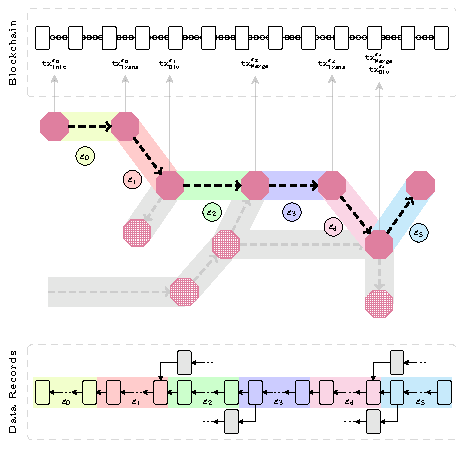
\includegraphics[width=.65\linewidth]{Figures/ZupplyNetwork}
    \caption{The lifecycle of a Product in the Zupply framework}
    \label{fig:enter-label}
\end{figure}

The Zupply framework is designed to ensure the integrity and authenticity of a product's historical data, represented as a \gls{dag}. 

This section describes how the Zupply framework can be employed in its main application i.e., \gls{scm}. Entities in our framework refer to participants in a supply chain — including producers, distributors, and retailers — who upload data records related to products. These entities have three primary objectives in this ecosystem: verifying the authenticity of previously uploaded data records, preserving the integrity of their data records over time, and maintaining their anonymity. Figure \ref{fig:enter-label} illustrates all three components of the Zupply framework in an example supply chain.

The initial entity in the supply chain, referred to as $e_{0}$ (e.g., a supplier of raw materials), creates an \gls{aat}, denoted as $T^{e_{0}}_{j_1}$. To accomplish this, $e_{0}$ executes the $\mathsf{Init}$ function, passing the product quantity ($q_{j_1}$) as an argument. Consequently, a new token, $T^{e_{0}}_{j_1}$, is generated, and its commitment, defined as $\texttt{cm}^{e_{0}}_{j_1} := \mathsf{COMM}_{\rho_{j_1}}(T^{e_{0}}_{j_1})$, is transmitted to the blockchain through a transaction termed $\texttt{tx}^{e_{0}}_\mathsf{Init}$. Then updates its localized version of the \textsf{MHT}, and also updates the root $\texttt{rt}_\tau$ on the smart contract ($\mathcal{C}_Z$). The smart contract verifies the correctness of the new root accordingly (as explained in Section \ref{sec:MerkleTreeStructure}). Following this, entity $e_0$ can begin uploading data records to the \gls{dcs} by utilizing the $\mathsf{Upload}$ function. This function employs a public parameters, referred to as $\textsc{pp}$, to establish a \gls{zkp}, proving the ownership of an authentication token in \textsf{MHT}. Moreover, each data record is signed using a private key, denoted as \( \text{SKsig}^{e_{0}}_{{j_1}} \). $\text{SKsig}_{i}$ and its corresponding $\text{PKsig}_{i}$ are included in \( T^{e_{0}}_{j_1} \) (see Section \ref{sec:zupply-terms-and-concepts}). This ensures the authenticity and integrity of the data.


% , which its corresponding public key \( \text{PKsig}^{e_{0}}_{{j_1}} \) is included in \( T^{e_{0}}_{j_1} \). This ensures the authenticity and integrity of the data.

In supply chains, a product is transferred among various entities, and each entity needs to transfer the ownership of the products they possess. If the entity $e_{0}$ wants to give a batch of products to the next entity $e_{1}$ and the corresponding \gls{aat} to the batch is $T^{e_{0}}_{j_1}$, the entity executes $\mathsf{Trans}$ algorithm, passing the \gls{aat} as one of its arguments. The algorithm generates a new $\Tilde{T}^{e_{1}}_{j_2}$ for the batch and passes it to $e_{1}$ in a secure off chain channel and submits transaction $\texttt{tx}^{e_{0}}_\mathsf{Trans}$ to the blockchain (the \gls{aat} ownership transfer protocol, i.e., \textsf{OT-Protocol}, is presented in Section \ref{sec:Ownership Transfer}). According to the \textsf{OT-Protocol}, $e_{0}$ cannot use $\Tilde{T}^{e_{1}}_{j_2}$ to upload data records since it does not know the corresponding $\text{SKsig}^{e_{1}}_{j_2}$. The transaction $\texttt{tx}^{e_{0}}_\mathsf{Trans}$ contains a \gls{zkp} of four things: (1) knowing the pre-image of the $\texttt{cm}_{j_1}^{e_{0}}$ which is in the \textsf{MHT} without revealing $\texttt{cm}_{j_1}^{e_{0}}$, (2) the included $\texttt{eol}$ in the transaction is related to  $\texttt{cm}_{j_1}^{e_{0}}$, (3) the proof of knowledge of $\Tilde{T}^{e_{1}}_{j_2}$ related to $\texttt{cm}^{e_{1}}_{j_2} := \mathsf{COMM}_\rho(T^{e_{i_2}}_{j_2})$ included in the transaction (4) the quantity $q_{j_2}=q_{j_1}$ does not change.

In the Zupply framework, entities can split a single authentication token into two using the \textsf{Div} algorithm. For instance, ${e_{1}}$ receives a batch from ${e_{0}}$ and decides to divide it into two smaller batches. One batch is sent to entity ${e_{2}}$, while the other is transferred to a different supply chain. Importantly, both supply chains should be able to access the product's history prior to this division. Additionally, entities have the ability to merge two of their authentication tokens into one using the \textsf{Merge} algorithm. For example, ${e_{2}}$ receives some products from a different supply chain and seeks to batch them together before passing them to ${e_{3}}$. Furthermore, auditors should have the capability to access and review the data records pertaining to both merged supply chains. These functionalities allow for the merging and dividing of data sequences associated with the \gls{aat}s, thereby enabling the maintenance of data in a \gls{dag} structure within the framework.



\subsection{Business Contracts}
\label{App:Business Contracts}


Employing smart contract-enabled blockchain platforms for managing \gls{aat} in the Zupply framework can enable business smart contracts that employ Zupply smart contract $\mathcal{C}_Z$ as a lower layer of their operations. Business smart contracts can provide financial security for entities so they will not rely on a trusted third party for their payments. One example of a business contract is transferring funds upon delivering a product (i.e., transferring an \gls{aat}). Here, we are going to present an example of a business contract $\mathcal{C}_B$ that checks whether a specific \texttt{cm} is uploaded to $\mathcal{C}_Z$ or not. Then, it transfers the funds that were locked in $\mathcal{C}_B$.

In this example, $e_1$ wants to send a product to $e_3$ via $e_2$. $e_2$ uploads data collected from the product till it transfers that to $e_3$. Later on, $e_3$ is going to continue uploading data records related to the product. $e_2$ wants a guaranteed payment by the time the product is delivered to $e_3$. Therefore, any entity who is responsible for the payment ($e_1$ in this example) can lock some funds in $\mathcal{C}_B$. The funds will be transferred to $e_2$ if the entity uploads an \gls{aat} commitment \texttt{cm}, which has been determined at the time of locking the funds to $\mathcal{C}_B$.


The followings are the steps of the the protocol:
\begin{enumerate}
    \item $(\text{PKsig}^{e_3}_1, \text{SKsig}^{e_3}_1) \leftarrow {e_3}^{\mathcal{K}_\mathsf{sig}}(\textsc{pp})$

    \item $e_3$ passes $\text{PKsig}^{e_3}_1$ to $e_1$.

    \item $e_2$: $\rho \xleftarrow{R} \{0, 1\}^O(\lambda)$

    \item $e_2$ passes $\rho$ to $e_1$ upon receiving the product from $e_1$.

    \item $e_1$ creates $\Tilde{T} = (q, \text{PKsig}^{e_3}_{1}, \rho)$ $\texttt{cm} \gets \mathsf{COMM}_\rho(\Tilde{T})$

    \item $e_1$ locks some funds in $\mathcal{C}_B$. These funds will go to $e_2$ whenever \texttt{cm} is uploaded to $\mathcal{C}_Z$ in a $\texttt{tx}_\mathsf{Trans}$ transactions.

    \item Upon receiving the product by $e_3$, both $e_2$ and $e_3$ will engage in the \textsf{OT-Protocol} presented in Section \ref{sec:Ownership Transfer}. $e_3$ will send $\text{PKsig}^{e_3}_1$ to $e_2$ after receiving ``Public key request'' from $e_2$ in the protocol.

    \item $e_2$ uses $\rho$ received from $e_1$ at the time of taking the product and  $\text{PKsig}^{e_3}_1$ received from $e_3$ at the time of giving product. Then outputs a new authentication token commitment \texttt{cm} via \textsf{Trans} algorithm.

    \item In the previous step \texttt{cm} is uploaded to the $\mathcal{C}_Z$ contract; therefore, $e_2$ can take the funds from $\mathcal{C}_B$.
    
\end{enumerate}

\subsection{Data Encryption}
\label{app:Data Encryption}
In the Zupply framework, various key management schemes can be employed to encrypt the private parts of the data records, adapting them according to different applications. In this thesis, we suggest following the Mesh forward secrecy approach for generating keys \cite{altawy2019mesh}. Such that the secret keys $\textsc{k}$ are generated by the radio frequency identification (RFID) tag's Pseudo-random bit generator (PRBG). This approach ensures that, in supply chain applications, a new product owner must have access to all previous encryption keys to trace the product's history effectively. However, it should not be able to decrypt the future data records after the point of transfer to the following entity. Ultimately, the final entity in the supply chain can view the complete history of the associated data progressive chain.


\section{Summary}
\label{app:zupply-summary}


Transferring applications such as \gls{scm}  to permissionless (public) blockchains eliminates the need for trust in a manager and offers a range of benefits, which we will discuss later in this paper. However, by the nature of permissionless blockchain, miners, monitors, auditors and validators see the plain transactions on the blockchain.  This could reveal the privacy of the data providers  and actors in  ownership transfer  of the data from one to another.  However, those will expose inventory information of different business sectors.  So, for blockchain based \gls{scm}, the privacy of data uploader (anonymous problem), and ownership transfer of data (unlinkable problem) is a crucial factor to deploy this technology. 

This chapter proposed a novel anonymous authentication token (\gls{aat}) framework that supports unlinkable \gls{aat} ownership transfer (\gls{aatot}) including unlinkable merging and dividing of \gls{aat}s, realized by \textsf{OT-Protocol} to ensure unlinkability during ownership transfer. The construction leverages zero-knowledge proof (\gls{zkp}) protocols to guarantee anonymity, unlinkability, and authentication. Building on this foundation, we introduce Zupply, a decentralized framework for maintaining directed acyclic graphs (\gls{dag}s) of authentic data records. Designed on a permissionless, smart contract-enabled blockchain, Zupply provides a trustless framework that preserves anonymity and unlinkability among participants while ensuring the integrity and authenticity of data records throughout the supply chain. Its efficiency is realized by minimizing the number of public inputs to the ZKPs, and the \textsf{MHT-Protocol} which updates the root of the MHT on the $\mathcal{C}_Z$  and eliminate the need for storing the entire tree on-chain. 



Zupply adopted a stricter adversary model that previous methods, in which the underlying blockchain platform does not preserve the anonymity of the transaction issuer (adversary's access to $\mathcal{O}^\mathsf{Attr}$). Moreover, transactions scale independently of participant count, Zupply requires no centralized servers or layer-1 changes, and let auditors focus only on relevant records. In contrast, zkLedger \cite{zkLedger2018}has to involve all entities per transaction, Mesh \cite{altawy2019mesh} lacks unlinkability and needs a central server, and DECOUPLES \cite{Maouchi2019DECOUPLES} modifies the base blockchain. 